% Options for packages loaded elsewhere
\PassOptionsToPackage{unicode}{hyperref}
\PassOptionsToPackage{hyphens}{url}
%
\documentclass[
]{article}
\usepackage{amsmath,amssymb}
\usepackage{iftex}
\ifPDFTeX
  \usepackage[T1]{fontenc}
  \usepackage[utf8]{inputenc}
  \usepackage{textcomp} % provide euro and other symbols
\else % if luatex or xetex
  \usepackage{unicode-math} % this also loads fontspec
  \defaultfontfeatures{Scale=MatchLowercase}
  \defaultfontfeatures[\rmfamily]{Ligatures=TeX,Scale=1}
\fi
\usepackage{lmodern}
\ifPDFTeX\else
  % xetex/luatex font selection
\fi
% Use upquote if available, for straight quotes in verbatim environments
\IfFileExists{upquote.sty}{\usepackage{upquote}}{}
\IfFileExists{microtype.sty}{% use microtype if available
  \usepackage[]{microtype}
  \UseMicrotypeSet[protrusion]{basicmath} % disable protrusion for tt fonts
}{}
\makeatletter
\@ifundefined{KOMAClassName}{% if non-KOMA class
  \IfFileExists{parskip.sty}{%
    \usepackage{parskip}
  }{% else
    \setlength{\parindent}{0pt}
    \setlength{\parskip}{6pt plus 2pt minus 1pt}}
}{% if KOMA class
  \KOMAoptions{parskip=half}}
\makeatother
\usepackage{xcolor}
\usepackage[margin=1in]{geometry}
\usepackage{color}
\usepackage{fancyvrb}
\newcommand{\VerbBar}{|}
\newcommand{\VERB}{\Verb[commandchars=\\\{\}]}
\DefineVerbatimEnvironment{Highlighting}{Verbatim}{commandchars=\\\{\}}
% Add ',fontsize=\small' for more characters per line
\usepackage{framed}
\definecolor{shadecolor}{RGB}{248,248,248}
\newenvironment{Shaded}{\begin{snugshade}}{\end{snugshade}}
\newcommand{\AlertTok}[1]{\textcolor[rgb]{0.94,0.16,0.16}{#1}}
\newcommand{\AnnotationTok}[1]{\textcolor[rgb]{0.56,0.35,0.01}{\textbf{\textit{#1}}}}
\newcommand{\AttributeTok}[1]{\textcolor[rgb]{0.13,0.29,0.53}{#1}}
\newcommand{\BaseNTok}[1]{\textcolor[rgb]{0.00,0.00,0.81}{#1}}
\newcommand{\BuiltInTok}[1]{#1}
\newcommand{\CharTok}[1]{\textcolor[rgb]{0.31,0.60,0.02}{#1}}
\newcommand{\CommentTok}[1]{\textcolor[rgb]{0.56,0.35,0.01}{\textit{#1}}}
\newcommand{\CommentVarTok}[1]{\textcolor[rgb]{0.56,0.35,0.01}{\textbf{\textit{#1}}}}
\newcommand{\ConstantTok}[1]{\textcolor[rgb]{0.56,0.35,0.01}{#1}}
\newcommand{\ControlFlowTok}[1]{\textcolor[rgb]{0.13,0.29,0.53}{\textbf{#1}}}
\newcommand{\DataTypeTok}[1]{\textcolor[rgb]{0.13,0.29,0.53}{#1}}
\newcommand{\DecValTok}[1]{\textcolor[rgb]{0.00,0.00,0.81}{#1}}
\newcommand{\DocumentationTok}[1]{\textcolor[rgb]{0.56,0.35,0.01}{\textbf{\textit{#1}}}}
\newcommand{\ErrorTok}[1]{\textcolor[rgb]{0.64,0.00,0.00}{\textbf{#1}}}
\newcommand{\ExtensionTok}[1]{#1}
\newcommand{\FloatTok}[1]{\textcolor[rgb]{0.00,0.00,0.81}{#1}}
\newcommand{\FunctionTok}[1]{\textcolor[rgb]{0.13,0.29,0.53}{\textbf{#1}}}
\newcommand{\ImportTok}[1]{#1}
\newcommand{\InformationTok}[1]{\textcolor[rgb]{0.56,0.35,0.01}{\textbf{\textit{#1}}}}
\newcommand{\KeywordTok}[1]{\textcolor[rgb]{0.13,0.29,0.53}{\textbf{#1}}}
\newcommand{\NormalTok}[1]{#1}
\newcommand{\OperatorTok}[1]{\textcolor[rgb]{0.81,0.36,0.00}{\textbf{#1}}}
\newcommand{\OtherTok}[1]{\textcolor[rgb]{0.56,0.35,0.01}{#1}}
\newcommand{\PreprocessorTok}[1]{\textcolor[rgb]{0.56,0.35,0.01}{\textit{#1}}}
\newcommand{\RegionMarkerTok}[1]{#1}
\newcommand{\SpecialCharTok}[1]{\textcolor[rgb]{0.81,0.36,0.00}{\textbf{#1}}}
\newcommand{\SpecialStringTok}[1]{\textcolor[rgb]{0.31,0.60,0.02}{#1}}
\newcommand{\StringTok}[1]{\textcolor[rgb]{0.31,0.60,0.02}{#1}}
\newcommand{\VariableTok}[1]{\textcolor[rgb]{0.00,0.00,0.00}{#1}}
\newcommand{\VerbatimStringTok}[1]{\textcolor[rgb]{0.31,0.60,0.02}{#1}}
\newcommand{\WarningTok}[1]{\textcolor[rgb]{0.56,0.35,0.01}{\textbf{\textit{#1}}}}
\usepackage{longtable,booktabs,array}
\usepackage{calc} % for calculating minipage widths
% Correct order of tables after \paragraph or \subparagraph
\usepackage{etoolbox}
\makeatletter
\patchcmd\longtable{\par}{\if@noskipsec\mbox{}\fi\par}{}{}
\makeatother
% Allow footnotes in longtable head/foot
\IfFileExists{footnotehyper.sty}{\usepackage{footnotehyper}}{\usepackage{footnote}}
\makesavenoteenv{longtable}
\usepackage{graphicx}
\makeatletter
\def\maxwidth{\ifdim\Gin@nat@width>\linewidth\linewidth\else\Gin@nat@width\fi}
\def\maxheight{\ifdim\Gin@nat@height>\textheight\textheight\else\Gin@nat@height\fi}
\makeatother
% Scale images if necessary, so that they will not overflow the page
% margins by default, and it is still possible to overwrite the defaults
% using explicit options in \includegraphics[width, height, ...]{}
\setkeys{Gin}{width=\maxwidth,height=\maxheight,keepaspectratio}
% Set default figure placement to htbp
\makeatletter
\def\fps@figure{htbp}
\makeatother
\setlength{\emergencystretch}{3em} % prevent overfull lines
\providecommand{\tightlist}{%
  \setlength{\itemsep}{0pt}\setlength{\parskip}{0pt}}
\setcounter{secnumdepth}{-\maxdimen} % remove section numbering
\usepackage{amsmath}
\ifLuaTeX
  \usepackage{selnolig}  % disable illegal ligatures
\fi
\usepackage{bookmark}
\IfFileExists{xurl.sty}{\usepackage{xurl}}{} % add URL line breaks if available
\urlstyle{same}
\hypersetup{
  pdftitle={區塊鏈上代幣分派嘅全新提案:鑄造證明},
  pdfauthor={公平啟動實驗室(F.L.L.)},
  hidelinks,
  pdfcreator={LaTeX via pandoc}}

\title{區塊鏈上代幣分派嘅全新提案:鑄造證明}
\author{公平啟動實驗室(F.L.L.)}
\date{2024年11月6號}

\begin{document}
\maketitle

\subsubsection{摘要}\label{ux6458ux8981}

公平鑄造(或者叫公平啟動)嘅概念喺區塊鏈社群入面好受關注,但佢面對一啲關鍵問題,例如女巫攻擊、社群共識建立時間唔夠、詐騙同埋缺乏市場價值管理。

呢份文件提出一個新嘅解決方案------鑄造證明(PoM),靈感嚟自比特幣嘅挖礦難度機制。PoM旨在透過將算力轉化為鑄造參與度,解決公平性嘅問題,從而減輕女巫攻擊嘅影響,並為社群共識嘅建立提供充足時間。

提出嘅PoM設計旨在確保穩定嘅鑄造過程,抑止投機同欺詐行為,激勵真正嘅用戶。文件詳細分析PoM機制,包括計算難度係數同每個週期鑄造規模嘅核心公式等。

文件仲展示咗模擬測試參數同結果,顯示PoM喺維持穩定鑄造曲線方面嘅有效性。此外,仲討論咗基於時代、週期同減少因子嘅總供應量計算,以及預計嘅總鑄造時間。

呢份文件提出咗公平鑄造範式嘅重大進步,提供一個更公平、更以社群為導向嘅代幣鑄造同分派方式。PoM有潛力重塑去中心化金融嘅格局,確保更公平、更可持續嘅鑄造過程。

\subsection{1 - 問題}\label{ux554fux984c}

過去兩年,區塊鏈社群入面嘅公平鑄造(或公平啟動)變得極受歡迎。好多代幣好快完成咗鑄造過程,隨後喺去中心化交易所上市交易。不過,佢哋嘅價格走勢通常呈現一個共通模式:一開始快速上漲後,價格持續唔斷下跌。

經過兩年對唔同公平鑄造平台同項目嘅觀察同研究,我哋發現咗以下問題:

\subsubsection{1.1 - 女巫攻擊}\label{ux5973ux5debux653bux64ca}

根據相關數據,此類公平鑄造遊戲嘅真實參與者比例高達90\%。但令人震驚嘅係,超過95\%嘅代幣實際上由少數精通區塊鏈技術嘅人鑄造。因此,絕大多數普通真實參與者只能攞到好少量嘅代幣。

呢種技術方法通常被稱為``女巫攻擊'',佢剝奪咗公平鑄造嘅``公平性''。少數人以極低成本控制咗大量代幣,佢哋透過迅速推高代幣價格然後高價拋售來操縱市場,攞取巨額利潤,呢個行為被稱為``拉高拋售''。

\subsubsection{1.2 -
建立共識時間唔夠}\label{ux5efaux7acbux5171ux8b58ux6642ux9593ux5514ux5920}

社群缺乏足夠時間去建立共識。由於代幣鑄造速度好快,價格往往喺社群仲喺建設過程時就開始下跌,導致社群共識瓦解,最終令社群解散。

\subsubsection{1.3 - 詐騙}\label{ux8a50ux9a19}

一啲項目嘅成員透過技術手段親自參與鑄造,製造市場``熱烈''嘅假象,攞低成本代幣,操縱市場以攞取巨額利潤,將公平鑄造變成詐騙工具。

\subsubsection{1.4 -
缺乏市場價值管理(MVM)}\label{ux7f3aux4e4fux5e02ux5834ux50f9ux503cux7ba1ux7406mvm}

缺乏有效嘅市場價值管理措施。鑑於鑄造速度極快,而且通常100\%嘅代幣直接(或喺鑄造完成後)進入流通,市場價值管理變得至關重要。不過,與公平鑄造相關嘅代幣嘅``無主''特性要求社群自發組織MVM。可惜,由於鑄造速度過快,MVM往往喺代幣價格崩盤前無法及時實施。

\subsubsection{1.5 -
流動性管理係咪有效?}\label{ux6d41ux52d5ux6027ux7ba1ux7406ux4fc2ux54aaux6709ux6548}

一啲公平鑄造平台引入咗流動性管理機制,例如喺鑄造時收取一定費用,呢啲費用被鎖定喺智能合約入面,並喺滿足某些條件(例如達到目標金額或完成所有鑄造)後自動添加到去中心化交易所嘅流動性池。

但我哋觀察到,喺呢啲項目嘅初始價格快速上漲期間,流動性池入面嘅資金佔總流動性池嘅比例好低;當價格下跌時,流動性池入面嘅資金遠遠唔夠抵擋拋售。

\subsubsection{1.6 -
時間鎖係咪有效?}\label{ux6642ux9593ux9396ux4fc2ux54aaux6709ux6548}

一啲智能合約引入咗時間鎖以防止女巫攻擊,呢個真係可以防止用同一帳戶進行批量鑄造,但仍然無法阻止用唔同帳戶進行批量鑄造嘅參與者。

\subsubsection{1.7 -
內存池同最大可提取價值(MEV)}\label{ux5167ux5b58ux6c60ux540cux6700ux5927ux53efux63d0ux53d6ux50f9ux503cmev}

大多數區塊鏈基於以太坊EVM,EVM嘅內存池允許大量機械人``窺探''用戶喺新區塊打包前嘅意圖,並優先進行鏈上操作,例如鑄造同交易。我哋觀察到,喺以太坊(區塊打包間隔大約12秒)同Arbitrum等二層網絡(區塊打包間隔大約0.25秒)上存在大量呢類行為。呢啲行為被稱為``最大可提取價值(MEV)''。據估計,自2020年1月1日起,MEV總額已超過7.3億美元,大部分流向咗機械人同礦工。MEV嘅存在係由技術驅動,雖然可以理解,但極大影響咗鏈上操作嘅公平性。

我哋認為,有效防止女巫攻擊等技術手段同為社群共識嘅建立提供充足時間,已成為最嚴峻嘅挑戰。雖然好多公平鑄造平台已經意識到呢個問題嘅嚴重性,並試圖採取相應措施防止各種形式嘅欺詐,但實際效果相當有限。

為咗有效防止女巫攻擊,一啲平台或項目採用咗如KYC認證或依賴項目團隊控制嘅服務器提供授權簽名等技術,要求鑄造者持有呢個簽名先可以鑄造。但呢啲方法過於中心化,因此難以被加密社群廣泛接受同支持。

\subsection{2 - 提案}\label{ux63d0ux6848}

我哋認為,鑑於當前嘅區塊鏈技術,要完全消除呢啲問題好困難。但一啲新機制可以緩解呢啲問題並增強公平鑄造嘅公平性,建立更好嘅社群。

呢份文件提出以下解決方案:

\subsubsection{2.1 -
比特幣挖礦難度機制}\label{ux6bd4ux7279ux5e63ux6316ux7926ux96e3ux5ea6ux6a5fux5236}

呢個提案借鑑咗比特幣挖礦嘅難度機制,因此喺介紹提案之前,我哋先簡要介紹比特幣挖礦機制。

比特幣挖礦嘅難度機制係比特幣網絡嘅核心組成部分。佢確保喺去中心化網絡中,鑄造進度保持喺大約每10分鐘生成一個區塊嘅穩定速度。呢個機制旨在適應網絡算力喺唔同時間嘅變化,目標係無論加入網絡嘅節點點樣變化,新區塊嘅生成速度保持相對穩定。

比特幣挖礦難度嘅調整透過自動算法實現,大約每兩星期(2016個區塊)調整一次。呢個週期基於比特幣網絡嘅目標區塊生成時間(每10分鐘一個區塊)設計。如果過去2016個區塊嘅平均生成時間少於10分鐘,難度將會增加,以確保未來區塊生成時間返到10分鐘。反之,如果平均生成時間超過10分鐘,難度將會降低。

具體難度嘅計算基於前2016個區塊嘅生成時間同目標時間(20160分鐘,即兩星期)嘅比較。難度調整公式根據實際時間同目標時間嘅比例增加或減少難度。呢種調整係持續嘅,以確保比特幣網絡能夠適應唔斷變化嘅算力,無論係礦工加入或離開,或高算力嘅挖礦硬件參與。

此外,難度嘅調整仲受到最大變化限制,即單次調整嘅難度唔可以超過前次難度嘅4倍。呢個係為咗防止難度突然大幅波動影響網絡。

隨著比特幣網絡嘅發展,挖礦難度持續增加,主要原因係參與挖礦嘅算力唔斷增長。隨著越來越多礦工加入網絡同挖礦硬件技術嘅改進,挖礦總算力持續上升,呢個增加咗單個礦工或礦池發現新區塊嘅難度。因此,挖礦難度嘅增加反映咗比特幣網絡算力嘅增長,同時確保比特幣嘅發行速度保持穩定。

比特幣挖礦難度機制係比特幣網絡適應性同穩定性嘅關鍵。佢透過動態調整難度值,確保比特幣區塊生成速度保持喺設計目標水平,同時適應網絡算力嘅變化。

\paragraph{上述難度規則喺比特幣代碼中嘅關鍵代碼(C++版本)。}\label{ux4e0aux8ff0ux96e3ux5ea6ux898fux5247ux55baux6bd4ux7279ux5e63ux4ee3ux78bcux4e2dux5605ux95dcux9375ux4ee3ux78bccux7248ux672c}

\begin{Shaded}
\begin{Highlighting}[numbers=left,,]
\CommentTok{/* Calculate the difficulty for a given block index.}
\CommentTok{ */}
\DataTypeTok{double}\NormalTok{ GetDifficulty}\OperatorTok{(}\AttributeTok{const}\NormalTok{ CBlockIndex}\OperatorTok{\&}\NormalTok{ blockindex}\OperatorTok{)}
\OperatorTok{\{}
    \DataTypeTok{int}\NormalTok{ nShift }\OperatorTok{=} \OperatorTok{(}\NormalTok{blockindex}\OperatorTok{.}\NormalTok{nBits }\OperatorTok{\textgreater{}\textgreater{}} \DecValTok{24}\OperatorTok{)} \OperatorTok{\&} \BaseNTok{0xff}\OperatorTok{;}
    \DataTypeTok{double}\NormalTok{ dDiff }\OperatorTok{=}
        \OperatorTok{(}\DataTypeTok{double}\OperatorTok{)}\BaseNTok{0x0000ffff} \OperatorTok{/} \OperatorTok{(}\DataTypeTok{double}\OperatorTok{)(}\NormalTok{blockindex}\OperatorTok{.}\NormalTok{nBits }\OperatorTok{\&} \BaseNTok{0x00ffffff}\OperatorTok{);}

    \ControlFlowTok{while} \OperatorTok{(}\NormalTok{nShift }\OperatorTok{\textless{}} \DecValTok{29}\OperatorTok{)}
    \OperatorTok{\{}
\NormalTok{        dDiff }\OperatorTok{*=} \FloatTok{256.0}\OperatorTok{;}
\NormalTok{        nShift}\OperatorTok{++;}
    \OperatorTok{\}}
    \ControlFlowTok{while} \OperatorTok{(}\NormalTok{nShift }\OperatorTok{\textgreater{}} \DecValTok{29}\OperatorTok{)}
    \OperatorTok{\{}
\NormalTok{        dDiff }\OperatorTok{/=} \FloatTok{256.0}\OperatorTok{;}
\NormalTok{        nShift}\OperatorTok{{-}{-};}
    \OperatorTok{\}}

    \ControlFlowTok{return}\NormalTok{ dDiff}\OperatorTok{;}
\OperatorTok{\}}
\end{Highlighting}
\end{Shaded}

比特幣GitHub倉庫:\url{https://github.com/bitcoin/bitcoin/blob/1dda1892b6bcc3d4f9678960cc9e9920f491e87e/src/rpc/blockchain.cpp\#L87C1-L107C2}

\begin{Shaded}
\begin{Highlighting}[numbers=left,,]
\DataTypeTok{unsigned} \DataTypeTok{int}\NormalTok{ GetNextWorkRequired}\OperatorTok{(}\AttributeTok{const}\NormalTok{ CBlockIndex}\OperatorTok{*}\NormalTok{ pindexLast}\OperatorTok{,} \AttributeTok{const}\NormalTok{ CBlockHeader }\OperatorTok{*}\NormalTok{pblock}\OperatorTok{,} 
  \AttributeTok{const}\NormalTok{ Consensus}\OperatorTok{::}\NormalTok{Params}\OperatorTok{\&}\NormalTok{ params}\OperatorTok{)}
\OperatorTok{\{}
    \OtherTok{assert}\OperatorTok{(}\NormalTok{pindexLast }\OperatorTok{!=} \KeywordTok{nullptr}\OperatorTok{);}
    \DataTypeTok{unsigned} \DataTypeTok{int}\NormalTok{ nProofOfWorkLimit }\OperatorTok{=}\NormalTok{ UintToArith256}\OperatorTok{(}\NormalTok{params}\OperatorTok{.}\NormalTok{powLimit}\OperatorTok{).}\NormalTok{GetCompact}\OperatorTok{();}

    \CommentTok{// Only change once per difficulty adjustment interval}
    \ControlFlowTok{if} \OperatorTok{((}\NormalTok{pindexLast}\OperatorTok{{-}\textgreater{}}\NormalTok{nHeight}\OperatorTok{+}\DecValTok{1}\OperatorTok{)} \OperatorTok{\%}\NormalTok{ params}\OperatorTok{.}\NormalTok{DifficultyAdjustmentInterval}\OperatorTok{()} \OperatorTok{!=} \DecValTok{0}\OperatorTok{)}
    \OperatorTok{\{}
        \ControlFlowTok{if} \OperatorTok{(}\NormalTok{params}\OperatorTok{.}\NormalTok{fPowAllowMinDifficultyBlocks}\OperatorTok{)}
        \OperatorTok{\{}
            \CommentTok{// Special difficulty rule for testnet:}
            \CommentTok{// If the new block\textquotesingle{}s timestamp is more than 2* 10 minutes}
            \CommentTok{// then allow mining of a min{-}difficulty block.}
            \ControlFlowTok{if} \OperatorTok{(}\NormalTok{pblock}\OperatorTok{{-}\textgreater{}}\NormalTok{GetBlockTime}\OperatorTok{()} \OperatorTok{\textgreater{}}\NormalTok{ pindexLast}\OperatorTok{{-}\textgreater{}}\NormalTok{GetBlockTime}\OperatorTok{()} \OperatorTok{+}\NormalTok{ params}\OperatorTok{.}\NormalTok{nPowTargetSpacing}\OperatorTok{*}\DecValTok{2}\OperatorTok{)}
                \ControlFlowTok{return}\NormalTok{ nProofOfWorkLimit}\OperatorTok{;}
            \ControlFlowTok{else}
            \OperatorTok{\{}
                \CommentTok{// Return the last non{-}special{-}min{-}difficulty{-}rules{-}block}
                \AttributeTok{const}\NormalTok{ CBlockIndex}\OperatorTok{*}\NormalTok{ pindex }\OperatorTok{=}\NormalTok{ pindexLast}\OperatorTok{;}
                \ControlFlowTok{while} \OperatorTok{(}\NormalTok{pindex}\OperatorTok{{-}\textgreater{}}\NormalTok{pprev }\OperatorTok{\&\&}\NormalTok{ pindex}\OperatorTok{{-}\textgreater{}}\NormalTok{nHeight }\OperatorTok{\%}\NormalTok{ params}\OperatorTok{.}\NormalTok{DifficultyAdjustmentInterval}\OperatorTok{()} 
                  \OperatorTok{!=} \DecValTok{0} \OperatorTok{\&\&}\NormalTok{ pindex}\OperatorTok{{-}\textgreater{}}\NormalTok{nBits }\OperatorTok{==}\NormalTok{ nProofOfWorkLimit}\OperatorTok{)}
\NormalTok{                    pindex }\OperatorTok{=}\NormalTok{ pindex}\OperatorTok{{-}\textgreater{}}\NormalTok{pprev}\OperatorTok{;}
                \ControlFlowTok{return}\NormalTok{ pindex}\OperatorTok{{-}\textgreater{}}\NormalTok{nBits}\OperatorTok{;}
            \OperatorTok{\}}
        \OperatorTok{\}}
        \ControlFlowTok{return}\NormalTok{ pindexLast}\OperatorTok{{-}\textgreater{}}\NormalTok{nBits}\OperatorTok{;}
    \OperatorTok{\}}

    \CommentTok{// Go back by what we want to be 14 days worth of blocks}
    \DataTypeTok{int}\NormalTok{ nHeightFirst }\OperatorTok{=}\NormalTok{ pindexLast}\OperatorTok{{-}\textgreater{}}\NormalTok{nHeight }\OperatorTok{{-}} \OperatorTok{(}\NormalTok{params}\OperatorTok{.}\NormalTok{DifficultyAdjustmentInterval}\OperatorTok{(){-}}\DecValTok{1}\OperatorTok{);}
    \OtherTok{assert}\OperatorTok{(}\NormalTok{nHeightFirst }\OperatorTok{\textgreater{}=} \DecValTok{0}\OperatorTok{);}
    \AttributeTok{const}\NormalTok{ CBlockIndex}\OperatorTok{*}\NormalTok{ pindexFirst }\OperatorTok{=}\NormalTok{ pindexLast}\OperatorTok{{-}\textgreater{}}\NormalTok{GetAncestor}\OperatorTok{(}\NormalTok{nHeightFirst}\OperatorTok{);}
    \OtherTok{assert}\OperatorTok{(}\NormalTok{pindexFirst}\OperatorTok{);}

    \ControlFlowTok{return}\NormalTok{ CalculateNextWorkRequired}\OperatorTok{(}\NormalTok{pindexLast}\OperatorTok{,}\NormalTok{ pindexFirst}\OperatorTok{{-}\textgreater{}}\NormalTok{GetBlockTime}\OperatorTok{(),}\NormalTok{ params}\OperatorTok{);}
\OperatorTok{\}}
\end{Highlighting}
\end{Shaded}

比特幣GitHub倉庫:\url{https://github.com/bitcoin/bitcoin/blob/1dda1892b6bcc3d4f9678960cc9e9920f491e87e/src/pow.cpp\#L14}

\subsubsection{2.2 -
�铸造證明(PoM)}\label{ux94f8ux9020ux8b49ux660epom}

如果我哋將比特幣嘅算力計算換成鑄造行為,有效將算力轉化為鑄造參與度,就得到我哋提出嘅解決方案,叫做\textbf{鑄造證明},簡稱\textbf{PoM}。

假設我哋喺以太坊上部署\textbf{PoM},以太坊已經更新為\textbf{權益證明(PoS)}共識,平均區塊時間大約\textbf{12秒}。為咗實現鑄造過程嘅穩定性,我哋設計咗以下計劃:

\begin{itemize}
\item
  整個鑄造進程分為幾個\textbf{時代},每個\textbf{時代}包含幾個\textbf{週期}。
\item
  每個\textbf{週期}有一個難度係數(初始\textbf{週期}嘅難度係數為\textbf{1}),由前一個\textbf{週期}嘅實際運行時間決定,並決定當前區塊嘅鑄造規模。
\item
  每個週期有多次鑄造實例,同一週期內每次鑄造嘅\textbf{鑄造規模}相同。
\item
  每個\textbf{時代}內嘅\textbf{週期}嘅\textbf{目標鑄造規模}同\textbf{基礎鑄造規模}按照固定嘅\textbf{減少因子}遞減。
\item
  每次鑄造需要支付固定費用,呢個費用唔會隨着\textbf{時代}同\textbf{週期}嘅鑄造規模減少而改變。
\end{itemize}

\subsubsection{2.3 - 示例:}\label{ux793aux4f8b}

\paragraph{2.3.1 - 快速鑄造}\label{ux5febux901fux9444ux9020}

喺第一個\textbf{時代},\textbf{目標週期鑄造規模}為\textbf{100,000代幣},\textbf{基礎週期鑄造規模}為\textbf{100代幣},\textbf{目標週期鑄造時間}為\textbf{10分鐘},鑄造費用為\textbf{0.1
ETH}。

假設喺第九個\textbf{週期},喺400秒內鑄造咗\textbf{100,000代幣},\textbf{難度係數}為\textbf{1.015086348},第十個\textbf{週期}耗時200秒,噉第十個\textbf{週期}嘅\textbf{難度係數}將自動增加到\textbf{1.028665947},\textbf{每次鑄造嘅規模}將自動減少到\textbf{100
/ 1.028665947 = 97.86137759代幣},每代幣嘅成本為\textbf{0.1 ETH /
97.86137759代幣 = 0.001021854 ETH}。

跟住,第十一個\textbf{週期}耗時\textbf{1000分鐘}(超過目標時間600秒),因此\textbf{難度係數}將保持同第十個\textbf{週期}相同,即\textbf{1.02185359},\textbf{每次鑄造嘅規模}同每代幣嘅成本同第十個\textbf{週期}相同。

然後,第十六個\textbf{週期}嘅鑄造時間變為\textbf{200秒},\textbf{難度係數}將自動增加到\textbf{1.028665947},\textbf{每次鑄造嘅規模}將減少到\textbf{100
/ 1.028665947 = 97.213289代幣},每代幣嘅成本為\textbf{0.1 ETH /
97.213289代幣 = 0.001028666 ETH},高過之前嘅\textbf{週期}。

以下係解釋上述示例嘅表格:

\begin{longtable}[]{@{}
  >{\raggedright\arraybackslash}p{(\columnwidth - 10\tabcolsep) * \real{0.0603}}
  >{\raggedright\arraybackslash}p{(\columnwidth - 10\tabcolsep) * \real{0.1207}}
  >{\raggedright\arraybackslash}p{(\columnwidth - 10\tabcolsep) * \real{0.2845}}
  >{\raggedright\arraybackslash}p{(\columnwidth - 10\tabcolsep) * \real{0.1983}}
  >{\raggedright\arraybackslash}p{(\columnwidth - 10\tabcolsep) * \real{0.1983}}
  >{\raggedright\arraybackslash}p{(\columnwidth - 10\tabcolsep) * \real{0.1379}}@{}}
\toprule\noalign{}
\begin{minipage}[b]{\linewidth}\raggedright
週期
\end{minipage} & \begin{minipage}[b]{\linewidth}\raggedright
週期鑄造時間
\end{minipage} & \begin{minipage}[b]{\linewidth}\raggedright
難度係數變化
\end{minipage} & \begin{minipage}[b]{\linewidth}\raggedright
難度係數
\end{minipage} & \begin{minipage}[b]{\linewidth}\raggedright
每次鑄造規模
\end{minipage} & \begin{minipage}[b]{\linewidth}\raggedright
每代幣成本
\end{minipage} \\
\midrule\noalign{}
\endhead
\bottomrule\noalign{}
\endlastfoot
1 & 500 & 0.001666667 & 1.001666667 & 99.83361065 & 0.001001667 \\
2 & 400 & 0.003333333 & 1.005005556 & 99.50193752 & 0.001005006 \\
3 & 500 & 0.001666667 & 1.006680565 & 99.3363769 & 0.001006681 \\
4 & 600 & 0 & 1.006680565 & 99.3363769 & 0.001006681 \\
5 & 700 & 0 & 1.006680565 & 99.3363769 & 0.001006681 \\
6 & 800 & 0 & 1.006680565 & 99.3363769 & 0.001006681 \\
7 & 600 & 0 & 1.006680565 & 99.3363769 & 0.001006681 \\
8 & 400 & 0.003333333 & 1.010036167 & 99.00635571 & 0.001010036 \\
\textbf{9} & ascended & 0.005 & 1.015086348 & 98.51378678 &
0.001015086 \\
\textbf{10} & 200 & 0.006666667 & 1.02185359 & 97.86137759 &
0.001021854 \\
\textbf{11} & 1000 & 0 & 1.02185359 & 97.86137759 & 0.001021854 \\
12 & 800 & 0 & 1.02185359 & 97.86137759 & 0.001021854 \\
13 & 1200 & 0 & 1.02185359 & 97.86137759 & 0.001021854 \\
14 & 1500 & 0 & 1.02185359 & 97.86137759 & 0.001021854 \\
15 & 1000 & 0 & 1.02185359 & 97.86137759 & 0.001021854 \\
\textbf{16} & 200 & 0.006666667 & 1.028665947 & 97.213289 &
0.001028666 \\
17 & 800 & 0 & 1.028665947 & 97.213289 & 0.001028666 \\
18 & 500 & 0.001666667 & 1.03038039 & 97.05153644 & 0.00103038 \\
19 & 600 & 0 & 1.03038039 & 97.05153644 & 0.00103038 \\
20 & 500 & 0.001666667 & 1.032097691 & 96.89005302 & 0.001032098 \\
\end{longtable}

上述表格嘅代幣成本圖表如下:

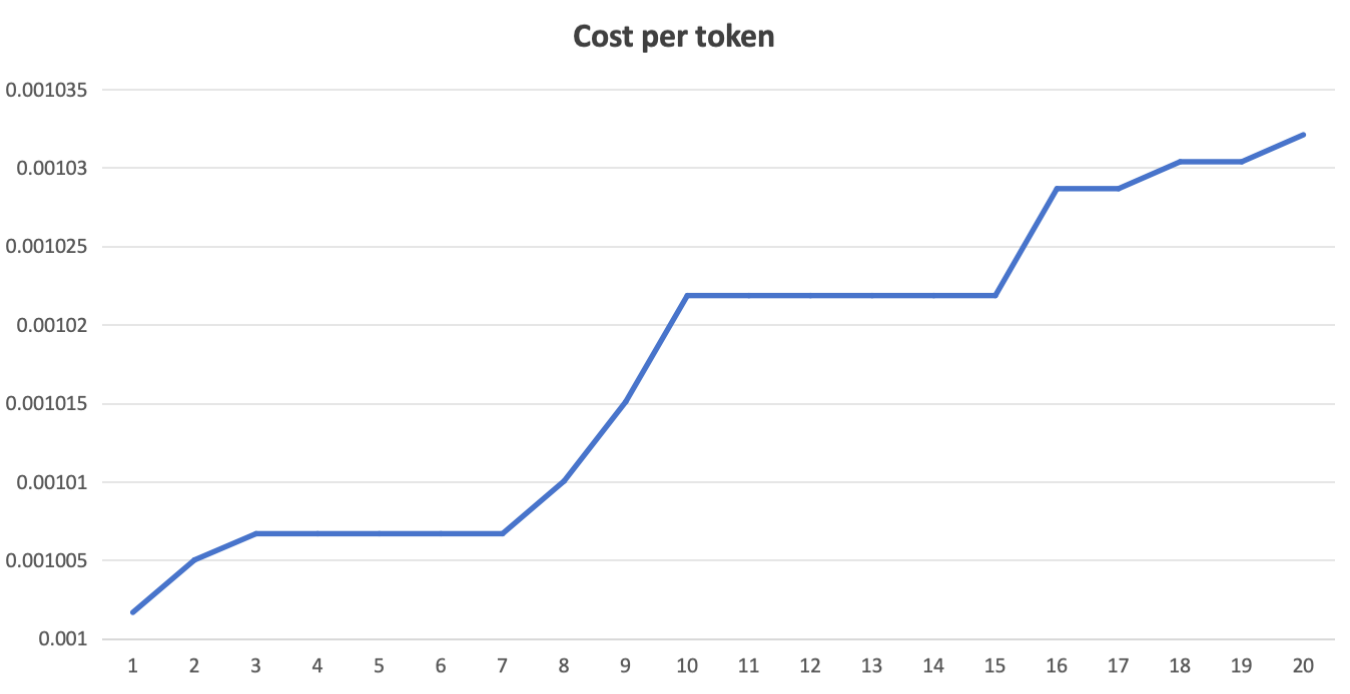
\includegraphics[width=400px]{image11}

\paragraph{2.3.1 -
按目標時間鑄造}\label{ux6309ux76eeux6a19ux6642ux9593ux9444ux9020}

如果鑄造速度太快,鑄造成本會好快上升。但如果按目標時間鑄造,每個人都會攞到相同嘅代幣成本。

以下係解釋嘅表格:

\begin{longtable}[]{@{}
  >{\raggedright\arraybackslash}p{(\columnwidth - 10\tabcolsep) * \real{0.0603}}
  >{\raggedright\arraybackslash}p{(\columnwidth - 10\tabcolsep) * \real{0.1207}}
  >{\raggedright\arraybackslash}p{(\columnwidth - 10\tabcolsep) * \real{0.2845}}
  >{\raggedright\arraybackslash}p{(\columnwidth - 10\tabcolsep) * \real{0.1983}}
  >{\raggedright\arraybackslash}p{(\columnwidth - 10\tabcolsep) * \real{0.1983}}
  >{\raggedright\arraybackslash}p{(\columnwidth - 10\tabcolsep) * \real{0.1379}}@{}}
\toprule\noalign{}
\begin{minipage}[b]{\linewidth}\raggedright
週期
\end{minipage} & \begin{minipage}[b]{\linewidth}\raggedright
週期鑄造時間
\end{minipage} & \begin{minipage}[b]{\linewidth}\raggedright
難度係數變化
\end{minipage} & \begin{minipage}[b]{\linewidth}\raggedright
難度係數
\end{minipage} & \begin{minipage}[b]{\linewidth}\raggedright
每次鑄造規模
\end{minipage} & \begin{minipage}[b]{\linewidth}\raggedright
每代幣成本
\end{minipage} \\
\midrule\noalign{}
\endhead
\bottomrule\noalign{}
\endlastfoot
1 & 589 & 0.000183333 & 1.000183333 & 99.98167003 & 0.001000183 \\
2 & 609 & 0 & 1.000183333 & 99.98167003 & 0.001000183 \\
3 & 596 & 6.66667E-05 & 1.000250012 & 99.97500503 & 0.00100025 \\
4 & 594 & 0.0001 & 1.000350037 & 99.96500853 & 0.00100035 \\
5 & 607 & 0 & 1.000350037 & 99.96500853 & 0.00100035 \\
6 & 609 & 0 & 1.000350037 & 99.96500853 & 0.00100035 \\
7 & 609 & 0 & 1.000350037 & 99.96500853 & 0.00100035 \\
8 & 608 & 0 & 1.000350037 & 99.96500853 & 0.00100035 \\
9 & 604 & 0 & 1.000350037 & 99.96500853 & 0.00100035 \\
10 & 608 & 0 & 1.000350037 & 99.96500853 & 0.00100035 \\
11 & 608 & 0 & 1.000350037 & 99.96500853 & 0.00100035 \\
12 & 607 & 0 & 1.000350037 & 99.96500853 & 0.00100035 \\
13 & 607 & 0 & 1.000350037 & 99.96500853 & 0.00100035 \\
14 & 605 & 0 & 1.000350037 & 99.96500853 & 0.00100035 \\
15 & 603 & 0 & 1.000350037 & 99.96500853 & 0.00100035 \\
16 & 589 & 0.000183333 & 1.000533435 & 99.94668497 & 0.001000533 \\
17 & 608 & 0 & 1.000533435 & 99.94668497 & 0.001000533 \\
18 & 590 & 0.000166667 & 1.00070019 & 99.93002996 & 0.0010007 \\
19 & 603 & 0 & 1.00070019 & 99.93002996 & 0.0010007 \\
20 & 611 & 0 & 1.00070019 & 99.93002996 & 0.0010007 \\
\end{longtable}

上述表格嘅代幣成本圖表如下:

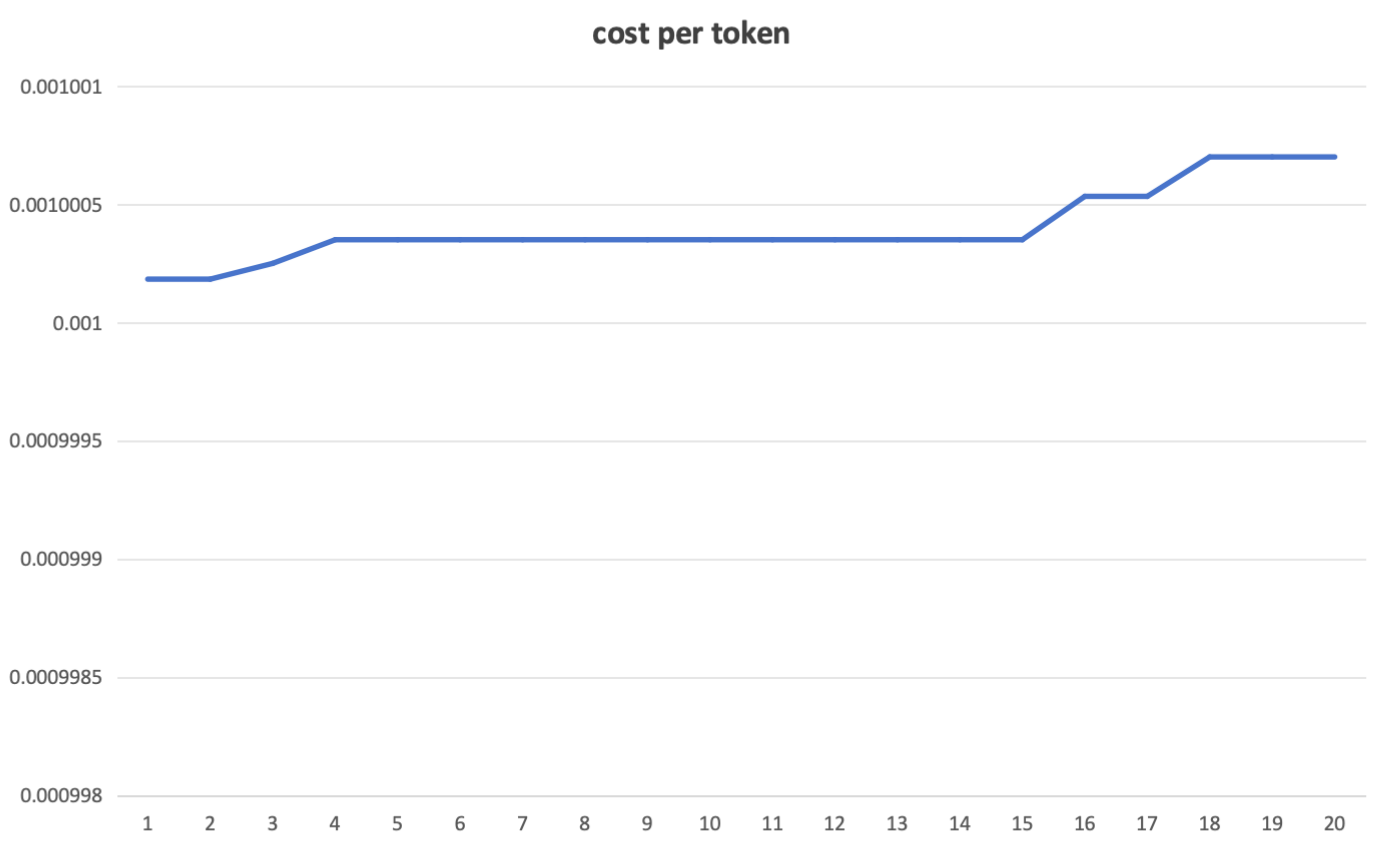
\includegraphics[width=400px]{image12}

\paragraph{2.3.2 -
關於週期基礎鑄造規模}\label{ux95dcux65bcux9031ux671fux57faux790eux9444ux9020ux898fux6a21}

另外,\textbf{週期基礎鑄造規模}會逐漸減少。假設\textbf{減少因子}為\textbf{3/4}:

\begin{itemize}
\item
  第一個\textbf{時代},\textbf{目標週期鑄造規模}為\textbf{100,000代幣},\textbf{週期基礎鑄造規模}為\textbf{100代幣}。
\item
  第二個\textbf{時代},\textbf{目標週期鑄造規模}為\textbf{100,000 * 3/4
  = 75,000代幣},\textbf{週期基礎鑄造規模}為\textbf{75代幣}。
\item
  第三個\textbf{時代},\textbf{目標週期鑄造規模}為\textbf{75,000 * 3/4 =
  56,250代幣},\textbf{週期基礎鑄造規模}為\textbf{56.25代幣}。
\item
  \ldots{}
\end{itemize}

\subsubsection{2.4 - 優勢}\label{ux512aux52e2}

\paragraph{2.4.1 - 優勢1}\label{ux512aux52e21}

如果\textbf{機械人}參與鑄造,佢哋會發現鑄造速度越快,攞到嘅代幣越少,成本越高。與好多試圖阻止\textbf{機械人}參與鑄造嘅方法相反,呢個提案唔阻止機械人進行批量鑄造。但高成本同低收益會阻止機械人。

\paragraph{2.4.2 - 優勢2}\label{ux512aux52e22}

如果\textbf{機械人}監控前一個\textbf{週期}嘅鑄造時間去計算下一個\textbf{週期}嘅難度同評估係咪參與,噉所有機械人必須有自己嘅策略。否則,趨同嘅策略會導致所有機械人一窩蜂,造成收益大幅下降同成本大幅上升。因為機械人嘅收益唔取決於鑄造嘅``速度'',而更多取決於對其他機械人行為嘅``猜測'',大大增加機械人嘅策略難度。

\paragraph{2.4.3 - 優勢3}\label{ux512aux52e23}

採用難度只增不減嘅機制,確保預期鑄造成本始終上升。當難度迅速增加時,用戶唔會期待難度下降,要唔係繼續鑄造,要唔係停止鑄造。呢個避免咗等待難度下降導致嘅鑄造停滯。

\paragraph{2.4.4 - 優勢4}\label{ux512aux52e24}

隨着難度同鑄造成本嘅增加,直到市場認為成本達到合理水平,鑄造會放緩或停止。呢個時候嘅鑄造成本會成為代幣市場價格嘅錨點。

\paragraph{2.4.5 - 優勢5}\label{ux512aux52e25}

從鑄造中收集嘅資金用於去中心化交易所嘅流動性池。呢個提案避免咗過去一啲平台收取嘅固定鑄造費用遠遠唔夠市場流動性需求嘅問題。隨着難度增加,每次鑄造嘅產出會減少,完成目標週期鑄造規模所需嘅鑄造次數會增加,從而提高鑄造費用。增加嘅鑄造費用會進入流動性池,為市場價值管理提供充足嘅流動性支持。

\paragraph{2.4.6 - 優勢6}\label{ux512aux52e26}

當市場價格下跌時,人哋會發現鑄造不再具有成本效益,導致鑄造活動放緩或停止。低成本供應嘅增加會減少或停止,避免咗價格下跌同代幣供應持續增加嘅``死亡螺旋''陷阱。如果有新鑄造者加入,難度同成本會再次上升。

\paragraph{2.4.7 - 優勢7}\label{ux512aux52e27}

鑄造成本同難度完全取決於市場參與,無中心化控制,喺去中心化環境中實現動態平衡。

\begin{quote}
\mbox{}%
\paragraph{\texorpdfstring{\textbf{喺最大利益原則嘅驅動下,最終鑄造速度會趨向目標設定,並實現納什均衡}。}{喺最大利益原則嘅驅動下,最終鑄造速度會趨向目標設定,並實現納什均衡。}}\label{ux55baux6700ux5927ux5229ux76caux539fux5247ux5605ux9a45ux52d5ux4e0bux6700ux7d42ux9444ux9020ux901fux5ea6ux6703ux8da8ux5411ux76eeux6a19ux8a2dux5b9aux4e26ux5be6ux73feux7d0dux4ec0ux5747ux8861}
\end{quote}

呢個機制有效激勵早期參與者,對持續關注嘅社群成員好友好,同時對投機者同透過技術手段作弊嘅人唔友好。

\begin{quote}
我哋喺以太坊測試網\textbf{sepolia}(\textbf{solidity})同\textbf{Solana}(\textbf{rust/anchor})開發網上編碼咗\textbf{PoM}鑄造算法,並會提供前端\textbf{Typescript}腳本畀社群測試,同時開源\textbf{python}語言模擬代碼。
\end{quote}

\subsection{3. 計算}\label{ux8a08ux7b97}

\subsubsection{3.1 - 公式}\label{ux516cux5f0f}

\paragraph{3.1.1 -
當前週期嘅難度係數}\label{ux7576ux524dux9031ux671fux5605ux96e3ux5ea6ux4fc2ux6578}

\begin{itemize}
\tightlist
\item
  \(d\):難度係數
\item
  \(d'\):前一週期嘅難度係數
\item
  \(\delta d\):難度係數變化
\item
  \(N_e\):已過去週期嘅區塊數
\item
  \(N_t\):每個週期嘅目標區塊數
\end{itemize}

難度係數嘅變化基於實際時間同目標時間嘅比例計算。我哋只考慮已過去區塊數低於每個週期目標區塊數嘅情況。公式如下:

\begin{equation}
\delta d = \frac{1-\frac{N_e}{N_t}}{100},(N_e < N_t)
\end{equation} \begin{equation}
\delta d = 0,(N_e \geq N_t)
\end{equation}

\textbf{注意}:喺上述公式中,100係用來控制難度增加比例喺一定閾值範圍內嘅因子。將佢設為100意味着難度增加嘅最大比例為1\%。如果設為50,則難度增加嘅最大比例為2\%。

喺得到難度係數變化後,當前週期嘅難度係數為:

\begin{equation}
d = d' * (1 + \delta d)
\end{equation}

對於可以準確獲取區塊時間戳嘅區塊鏈,上述\textbf{區塊數}可以換成\textbf{時間戳}。

\textbf{示例:}

喺2.3.1嘅示例中,每個\textbf{週期}嘅目標鑄造時間為600秒。喺\textbf{第十週期},鑄造耗時200秒,\textbf{第九週期}嘅\textbf{難度係數}為\textbf{1.015086348},所以\textbf{第十週期}嘅新\textbf{難度係數}將調整為:
\textbf{1.015086348 * ((1 - 200 / 600) / 100 + 1) = 1.02185359}。

喺\textbf{第十一週期},鑄造耗時1000秒,超過目標鑄造時間600秒,噉保持同\textbf{第十週期}相同嘅\textbf{難度係數},即\textbf{1.02185359}。

\paragraph{3.1.2 -
當前時代每次鑄造嘅基礎規模(Mb)}\label{ux7576ux524dux6642ux4ee3ux6bcfux6b21ux9444ux9020ux5605ux57faux790eux898fux6a21mb}

\begin{itemize}
\tightlist
\item
  \(M_b\):當前時代每次鑄造嘅基礎規模
\item
  \(M_0\):創世時代每次鑄造嘅基礎規模
\item
  \(f\):減少因子
\item
  \(e\):當前時代
\end{itemize}

\begin{equation}
M_b = M_0 * f^{e-1}
\end{equation}

\textbf{減少因子}

\begin{itemize}
\tightlist
\item
  \(f\)=0.5表示每個時代減少\textbf{50\%}(減半)
\item
  \(f\)=2/3表示每個時代減少\textbf{33.33\%}
\item
  \(f\)=3/4表示每個時代減少\textbf{25\%}
\item
  \(f\)=4/5表示每個時代減少\textbf{20\%}
\item
  \(f\)=5/6表示每個時代減少\textbf{1/6},等等。
\end{itemize}

\paragraph{3.1.3 -
當前時代每個週期嘅目標鑄造規模}\label{ux7576ux524dux6642ux4ee3ux6bcfux500bux9031ux671fux5605ux76eeux6a19ux9444ux9020ux898fux6a21}

\begin{itemize}
\tightlist
\item
  \(T\):當前時代每個週期嘅目標鑄造規模
\item
  \(T_0\):創世時代每個週期嘅目標鑄造規模
\item
  \(f\):減少因子
\item
  \(e\):當前時代
\end{itemize}

\begin{equation}
 T = T_0 * f^{e-1}
\end{equation}

\paragraph{3.1.4 -
當前週期每次鑄造嘅規模}\label{ux7576ux524dux9031ux671fux6bcfux6b21ux9444ux9020ux5605ux898fux6a21}

\begin{itemize}
\tightlist
\item
  \(M\):當前週期每次鑄造嘅規模
\item
  \(M_b\):當前時代每次鑄造嘅基礎規模
\item
  \(d\):難度係數
\end{itemize}

\begin{equation}
M = \frac{M_b}{d}
\end{equation}

\textbf{示例:}

喺2.3.1嘅示例中,當前時代嘅\textbf{每次鑄造嘅基礎規模}為\textbf{100代幣},\textbf{第十六週期}嘅\textbf{難度係數}為\textbf{1.028665947},噉鑄造規模為:\textbf{100
/ 1.028665947 = 97.213289代幣}。

\paragraph{3.1.5}\label{section}

如果\(T\)唔係\(M\)嘅整數倍,需要對\(M\)進行調整,即:

\begin{equation}
M_a = \frac{T}{\lfloor\frac{T}{M}\rfloor + 1}, (T \nmid M)
\end{equation}

如果\(T\)係\(M\)嘅整數倍,則唔需要如上調整。 \begin{equation}
M_a = M, (T \mid M)
\end{equation}

\paragraph{3.1.6 - 代幣成本}\label{ux4ee3ux5e63ux6210ux672c}

雖然每次鑄造嘅費用保持不變,但隨着難度增加,每次鑄造獲得嘅代幣數量會減少,因此代幣成本會增加。

以下係計算代幣成本嘅方法。

\begin{itemize}
\tightlist
\item
  \(P_0\):鑄造費用
\item
  \(p\):代幣成本
\end{itemize}

\begin{equation}
p = \frac{P_0}{M_a}
\end{equation} 如果\textbf{T}唔係\textbf{M}嘅整數倍,價格為:
\begin{equation}
p = \frac{P_0*(\lfloor\frac{T_0}{M_0}*d\rfloor + 1)}{T_0*f^{e-1}}, (T \nmid M)
\end{equation} \begin{equation}
p = \frac{P_0}{M_0*f^{e-1}}*d, (T \mid M)
\end{equation}
由於\(P_0\)、\(T_0\)、\(M_0\)、\(f\)同\(e\)喺一個時代內係常數,我哋知道:\(p \propto d\)。

\paragraph{3.1.7}\label{section-1}

\(T\)同\(M\)隨着每個\textbf{時代}呈指數減少,但兩者之間嘅比例保持不變,無論喺邊個\textbf{時代}。

\begin{equation}
T=T_0*f^{e-1}
\end{equation} \begin{equation}
M = \frac{M_b}{d}=\frac{M_0 * f^{e-1}}{d}
\end{equation} \begin{equation}
\frac{T}{M} = \frac{T_0}{M_0} * d
\end{equation}

\paragraph{3.1.8}\label{section-2}

如果\(N_t\)設為10分鐘,噉理論上每次鑄造嘅目標間隔時間為:600秒 / 33 =
18.18秒每次。

如果間隔時間較長,意味着完成一個\textbf{週期}嘅所有鑄造需要比計劃時間(10分鐘)更長,呢個意味着鑄造者較少,喺呢個情況下,難度降低,每次鑄造嘅獎勵增加。

反之,如果間隔時間較短,表明完成一個\textbf{週期}嘅鑄造時間少於計劃時間(10分鐘),呢個意味着鑄造者較多,喺呢個情況下,難度增加,每次鑄造嘅獎勵減少。

\subsubsection{3.2 -
計算週期鑄造規模嘅關鍵代碼(Rust)}\label{ux8a08ux7b97ux9031ux671fux9444ux9020ux898fux6a21ux5605ux95dcux9375ux4ee3ux78bcrust}

\begin{Shaded}
\begin{Highlighting}[numbers=left,,]
\KeywordTok{pub} \KeywordTok{fn}\NormalTok{ get\_mint\_size(}
\NormalTok{  config\_data}\OperatorTok{:} \OperatorTok{\&}\NormalTok{TokenConfigData}\OperatorTok{,}
\NormalTok{) }\OperatorTok{{-}\textgreater{}} \DataTypeTok{Result}\OperatorTok{\textless{}}\NormalTok{(}\DataTypeTok{u64}\OperatorTok{,} \DataTypeTok{f64}\OperatorTok{,} \DataTypeTok{u64}\NormalTok{)}\OperatorTok{\textgreater{}} \OperatorTok{\{}
  \KeywordTok{let}\NormalTok{ delta\_difficulty\_coefficient }\OperatorTok{=} \ControlFlowTok{if}\NormalTok{ config\_data}\OperatorTok{.}\NormalTok{mint\_state\_data}\OperatorTok{.}\NormalTok{elapsed\_seconds\_epoch}
    \OperatorTok{\textless{}}\NormalTok{ config\_data}\OperatorTok{.}\NormalTok{target\_seconds\_per\_epoch }\OperatorTok{\{}
\NormalTok{    (}\DecValTok{1.0} \OperatorTok{{-}}\NormalTok{ config\_data}\OperatorTok{.}\NormalTok{mint\_state\_data}\OperatorTok{.}\NormalTok{elapsed\_seconds\_epoch}\OperatorTok{.}\NormalTok{safe\_as\_f64()}\OperatorTok{?} \OperatorTok{/} 
\NormalTok{       config\_data}\OperatorTok{.}\NormalTok{target\_seconds\_per\_epoch}\OperatorTok{.}\NormalTok{safe\_as\_f64()}\OperatorTok{?}\NormalTok{) }\OperatorTok{/} \DecValTok{100.0}
  \OperatorTok{\}} \ControlFlowTok{else} \OperatorTok{\{}
    \DecValTok{0.0}
  \OperatorTok{\};}
  \KeywordTok{let}\NormalTok{ difficulty\_coefficient }\OperatorTok{=}\NormalTok{ config\_data}\OperatorTok{.}\NormalTok{mint\_state\_data}\OperatorTok{.}\NormalTok{difficulty\_coefficient\_epoch }
    \OperatorTok{*}\NormalTok{ (}\DecValTok{1.0} \OperatorTok{+}\NormalTok{ delta\_difficulty\_coefficient)}\OperatorTok{;}
  \KeywordTok{let}\NormalTok{ base\_mint\_size }\OperatorTok{=}\NormalTok{ config\_data}\OperatorTok{.}\NormalTok{initial\_mint\_size}\OperatorTok{.}\NormalTok{safe\_as\_f64()}\OperatorTok{?} 
    \OperatorTok{*}\NormalTok{ config\_data}\OperatorTok{.}\NormalTok{reduce\_ratio}\OperatorTok{.}\NormalTok{powf((config\_data}\OperatorTok{.}\NormalTok{mint\_state\_data}\OperatorTok{.}\NormalTok{current\_era }\OperatorTok{{-}} \DecValTok{1}\NormalTok{)}\OperatorTok{.}\NormalTok{safe\_as\_f64()}\OperatorTok{?}\NormalTok{)}\OperatorTok{;}
  \KeywordTok{let}\NormalTok{ base\_target\_mint\_size\_per\_epoch }\OperatorTok{=}\NormalTok{ config\_data}\OperatorTok{.}\NormalTok{initial\_target\_mint\_size\_per\_epoch}\OperatorTok{.}\NormalTok{safe\_as\_f64()}\OperatorTok{?} 
    \OperatorTok{*}\NormalTok{ config\_data}\OperatorTok{.}\NormalTok{reduce\_ratio}\OperatorTok{.}\NormalTok{powf((config\_data}\OperatorTok{.}\NormalTok{mint\_state\_data}\OperatorTok{.}\NormalTok{current\_era }\OperatorTok{{-}} \DecValTok{1}\NormalTok{)}\OperatorTok{.}\NormalTok{safe\_as\_f64()}\OperatorTok{?}\NormalTok{)}\OperatorTok{;}
  \KeywordTok{let}\NormalTok{ mint\_size }\OperatorTok{=}\NormalTok{  base\_mint\_size }\OperatorTok{/}\NormalTok{ difficulty\_coefficient}\OperatorTok{;}
  \KeywordTok{let}\NormalTok{ target\_mint\_size\_epoch }\OperatorTok{=}\NormalTok{ (base\_target\_mint\_size\_per\_epoch }\OperatorTok{/}\NormalTok{ mint\_size)}\OperatorTok{.}\NormalTok{trunc() }
  \OperatorTok{*}\NormalTok{ mint\_size}\OperatorTok{;}
  \ConstantTok{Ok}\NormalTok{((mint\_size}\OperatorTok{.}\NormalTok{safe\_as\_u64()}\OperatorTok{?,}\NormalTok{ difficulty\_coefficient}\OperatorTok{,}\NormalTok{ target\_mint\_size\_epoch}\OperatorTok{.}\NormalTok{safe\_as\_u64()}\OperatorTok{?}\NormalTok{))}
\OperatorTok{\}}
\end{Highlighting}
\end{Shaded}

\subsection{4. 部署參數}\label{ux90e8ux7f72ux53c3ux6578}

\subsubsection{4.1 總供應量}\label{ux7e3dux4f9bux61c9ux91cf}

同普通代幣發行模式唔同,\textbf{PoM}嘅\textbf{總供應量}基於\textbf{時代}、\textbf{週期}同\textbf{減少因子}計算。

確定總供應量嘅四個參數:

\begin{itemize}
\tightlist
\item
  \(E\):總時代數
\item
  \(C\):每個時代嘅週期數
\item
  \(T_0\):初始週期目標鑄造規模
\item
  \(f\):時代減少因子,\(f \in (0,1)\)
\end{itemize}

\textbf{計算}

\begin{equation}
TotalSupply = \sum_{i=1}^{E}(C \cdot T_0 \cdot f^{i-1})=C \cdot T_0 \cdot \frac{1-f^E}{1-f}
\end{equation}

\textbf{示例:}

\(E\)=15, \(C\)=10, \(T_0\)=100,000代幣, \(f\)=0.75

\textbf{總供應量為:} 3,946,546.156代幣

\href{https://www.wolframalpha.com/input?i=sum+10*100000*0.75\%5E\%28i-1\%29\%2C+i+\%3D+1+to+15}{點擊此處打開Wolfram計算},您可以用\textbf{Wolfram}輕鬆計算總供應量。

\paragraph{4.1.1 -
最大總供應量}\label{ux6700ux5927ux7e3dux4f9bux61c9ux91cf}

當\(E\)趨向無窮大,意味着鑄造可以無限期進行,\textbf{總供應量}會收斂到一個值,即:

\textbf{計算}

\begin{equation}
lim_{E→\infty}(\cdot C \cdot T_0\cdot\frac{1-f^E}{1-f})=C \cdot T_0\cdot \frac{1-f^{\infty}}{1-f}=\frac{C\cdot T_0}{1-f}
\end{equation}

\textbf{示例:}

\(C\)=10, \(T_0\)=100,000代幣, \(f\)=0.75

\textbf{總供應量為:} 4,000,000代幣

\subsubsection{4.2
預計總鑄造時間:}\label{ux9810ux8a08ux7e3dux9444ux9020ux6642ux9593}

\textbf{注意:} 實際總鑄造時間同預計總鑄造時間會有差別。

以下係計算預計總鑄造時間嘅公式。

\begin{itemize}
\tightlist
\item
  \(E\):時代
\item
  \(C\):每個時代嘅週期數
\item
  \(N_t\):每個週期嘅目標區塊數
\item
  \(t\):每個區塊嘅秒數
\end{itemize}

\textbf{計算}

\begin{equation}
TotalEstimatedTime = E \cdot C \cdot N_t \cdot t
\end{equation}

\textbf{示例:} \(E\)=15, \(C\)=10, \(N_t\)=50, \(t\)=12秒

\textbf{預計總鑄造時間:} 15 * 10 * 50 * 12 = 90,000秒 = 25小時

\subsubsection{4.3 總時代數}\label{ux7e3dux6642ux4ee3ux6578}

結合以上兩個公式,我哋可以計算當鑄造咗80\%總供應量(\(r\))時嘅總時代數\(E_r\)。

\begin{equation}
C \cdot T_0 \cdot \frac{1-f^{E_r}}{1-f} = \frac{C \cdot T_0}{1-f}*r
\end{equation} 從呢個方程,我哋得到: \begin{equation}
E_r = \log_f(1-r)
\end{equation}

\textbf{示例:}

\(r\)=80\%, \(f\)=0.75, 則
\(E_r\)=\(\log_{0.75}(1-0.8)=\frac{\ln0.2}{\ln0.75}=5.59\)。

呢個意味着喺第六個時代中期,80\%嘅總供應量會被鑄造。

如果\(C=10\),喺第56個週期(5.59*10),80\%嘅總供應量會被鑄造。

\subsubsection{4.4 總鑄造費用}\label{ux7e3dux9444ux9020ux8cbbux7528}

每次鑄造需要支付固定費用,但由於難度嘅增加,同一週期內嘅鑄造次數會增加,每次鑄造獲得嘅代幣數量會減少,因此總費用會相應增加。

\begin{quote}
\textbf{注意:} 呢啲鑄造費用會自動加入流動性池。
\end{quote}

\begin{itemize}
\tightlist
\item
  \(Fee\):總費用
\item
  \(P_0\):每次鑄造嘅費用
\item
  \(d\):難度係數
\item
  \(Q\):一個週期內嘅鑄造次數
\item
  \(T_0\):創世時代每個週期嘅目標鑄造規模
\item
  \(M_0\):創世時代每次鑄造嘅基礎規模
\item
  \(C_e\):已過去嘅週期數,\(C_e = E * C\)
\end{itemize}

一個週期內嘅鑄造次數:

\begin{equation}
Q = {\lfloor{\frac{T_0}{M_0}*d}\rfloor + 1}, (T_0 \nmid M_0)
\end{equation}

\begin{equation}
Q = \frac{T_0}{M_0}*d, (T_0 \mid M_0)
\end{equation} 為簡單起見,假設\(T_0 \mid M_0\),總費用為:

\begin{equation}
TotalFee = \sum_{i=1}^{C_e}(P_0 \cdot Q_i)=\sum_{i=1}^{C_e}(\frac{P_0 \cdot T_0}{M_0}*d_i)
\end{equation}

由於\(d_i = d_{i-1} \cdot (1 + \delta d_i)\),
\(\delta d \in [0,0.01]\)(見3.1.1),而且\(d_0=1\),總費用範圍為:

\begin{equation}
TotalFee \in [\frac{P_0 \cdot T_0}{M_0} \cdot \sum_{i=1}^{C_e}1^i, \frac{P_0 \cdot T_0}{M_0} \cdot 101 \cdot (1.01^{C_e}-1)]
\end{equation}

簡化後:

\begin{equation}
TotalFee \in [\frac{P_0 \cdot T_0}{M_0} \cdot C_e, \frac{P_0 \cdot T_0}{M_0} \cdot 101 \cdot (1.01^{C_e}-1)]
\end{equation}

\textbf{示例}

\(P_0=1\)美元, \(T_0=9000\), \(M_0=100\), \(d=1.5\),
\(C_e=300\),最低總費用為27,000美元,最高為169,096.2美元。

呢個表明,如果鑄造速度好快,週期內嘅實際鑄造時間(\(N_e\))少於目標時間(\(N_t\)),會導致難度同鑄造成本持續增加。因此,收集嘅總費用會比難度保持不變時高出\textbf{6.3}倍,而且隨着週期數增加,差異會更加顯著。

\subsubsection{4.5 使用案例}\label{ux4f7fux7528ux6848ux4f8b}

\paragraph{4.5.1}\label{section-3}

如果目標總供應量為2100萬(左右),可以有(但唔限於)以下參數組合:

\begin{longtable}[]{@{}
  >{\raggedright\arraybackslash}p{(\columnwidth - 22\tabcolsep) * \real{0.0833}}
  >{\raggedright\arraybackslash}p{(\columnwidth - 22\tabcolsep) * \real{0.0833}}
  >{\raggedright\arraybackslash}p{(\columnwidth - 22\tabcolsep) * \real{0.0833}}
  >{\raggedright\arraybackslash}p{(\columnwidth - 22\tabcolsep) * \real{0.0833}}
  >{\raggedright\arraybackslash}p{(\columnwidth - 22\tabcolsep) * \real{0.0833}}
  >{\raggedright\arraybackslash}p{(\columnwidth - 22\tabcolsep) * \real{0.0833}}
  >{\raggedright\arraybackslash}p{(\columnwidth - 22\tabcolsep) * \real{0.0833}}
  >{\raggedright\arraybackslash}p{(\columnwidth - 22\tabcolsep) * \real{0.0833}}
  >{\raggedright\arraybackslash}p{(\columnwidth - 22\tabcolsep) * \real{0.0833}}
  >{\raggedright\arraybackslash}p{(\columnwidth - 22\tabcolsep) * \real{0.0833}}
  >{\raggedright\arraybackslash}p{(\columnwidth - 22\tabcolsep) * \real{0.0833}}
  >{\raggedright\arraybackslash}p{(\columnwidth - 22\tabcolsep) * \real{0.0833}}@{}}
\toprule\noalign{}
\begin{minipage}[b]{\linewidth}\raggedright
\(C\)
\end{minipage} & \begin{minipage}[b]{\linewidth}\raggedright
\(T_0\)
\end{minipage} & \begin{minipage}[b]{\linewidth}\raggedright
\(M_0\)
\end{minipage} & \begin{minipage}[b]{\linewidth}\raggedright
\(f\)
\end{minipage} & \begin{minipage}[b]{\linewidth}\raggedright
\(N_t\)
\end{minipage} & \begin{minipage}[b]{\linewidth}\raggedright
\(t\)
\end{minipage} & \begin{minipage}[b]{\linewidth}\raggedright
總供應量
\end{minipage} & \begin{minipage}[b]{\linewidth}\raggedright
時代
\end{minipage} & \begin{minipage}[b]{\linewidth}\raggedright
週期
\end{minipage} & \begin{minipage}[b]{\linewidth}\raggedright
天數
\end{minipage} & \begin{minipage}[b]{\linewidth}\raggedright
最低總費用
\end{minipage} & \begin{minipage}[b]{\linewidth}\raggedright
最高總費用
\end{minipage} \\
\midrule\noalign{}
\endhead
\bottomrule\noalign{}
\endlastfoot
600 & 9000 & 1000 & 0.75 & 2000 & 12 & 2160萬 & 10.413 & 6248 & 1735.56
& 56,241 & 9.088e29 \\
500 & 11000 & 1000 & 0.75 & 500 & 12 & 2200萬 & 10.413 & 5206 & 361.57 &
57,277 & 3.49e25 \\
2500 & 1000 & 100 & 0.75 & 1000 & 0.4 & 1000萬 & 10.413 & 26032 & 120.5
& 260,320 & 3.15e115 \\
\end{longtable}

\textbf{注意:}

\begin{itemize}
\item
  \(Eras = \log_f(1-0.95)\),鑄造率為95\%
\item
  \(Epoches = Eras * C\)
\item
  \(days = Epoches * N_t * t / 3600 / 24\) =
  \(log_f(1-0.95) * C * N_t * t / 86400\)
\item
  由於\(f\)、\(t\)係固定嘅,總天數取決於\(C\)同\(N_t\)
\end{itemize}

\paragraph{4.5.2
如何計算所有參數}\label{ux5982ux4f55ux8a08ux7b97ux6240ux6709ux53c3ux6578}

我哋會根據以下條件嚟計算所有參數:

\begin{itemize}
\tightlist
\item
  總供應量
\item
  目標鑄造天數
\item
  最低總費用
\end{itemize}

常量為:

\begin{itemize}
\tightlist
\item
  總供應量:10,000,000
\item
  目標鑄造天數:180天,95\%嘅總供應量會被鑄造
\item
  目標鑄造費用:30,000美元
\item
  \(f\) = 0.75
\item
  \(T_0\) = 10,000
\item
  \(M_0\) = 1,000
\item
  \(t\)=0.4秒(用於Solana區塊鏈)
\end{itemize}

\textbf{計算}

1-
\(\because TotalSupply = C \cdot T_0 / (1-f)\),所以每個時代嘅初始週期數(C)為:

\(C = TotalSupply \cdot (1 - f) / T_0\) = 10,000,000*(1-0.75)/10000=250

2- 根據以下公式,我哋可以得到\(N_t = 14935\) \begin{equation}
C * N_t * t * \log_f(1-0.95) = 180天 * 86400秒/天
\end{equation}

3- 根據以下公式,我哋可以得到\(C_e = 2603\) \begin{equation}
C_e = Eras * C = \log_f(1-0.95) * C = 10.413 * 250 = 2603
\end{equation}

4-
我哋已經知道:\(T_0=10,000\),\(C_e=2603\),\(M_0=1000\),最低總費用公式:

\begin{equation}
\frac{P_0 * T_0 * (C_e+1)}{M_0} = P_0 * 10,000 * 2604 / 1000 = 300,000
\end{equation}

根據最低總費用公式,我哋可以得到\(P_0 = 11.52\)美元,呢個意味着每個代幣嘅最低價格為
\(P_0 / M_0 = 11.52 / 1000 = 0.01152\)美元

\href{https://docs.google.com/spreadsheets/d/1z4eO1k14noxTMcgADMc-I0xFXT0giMFPSBEGal4suvI/edit?usp=sharing}{點擊此處打開在線計算器}

\subsection{5. 測試同評估}\label{ux6e2cux8a66ux540cux8a55ux4f30}

以下係模擬測試嘅參數:

\begin{itemize}
\tightlist
\item
  鑄造間隔時間範圍:0-30秒隨機
\item
  總時代數:10
\item
  每個時代嘅週期數:20
\item
  最低難度係數:0.2
\item
  減少係數:3/4
\item
  創世時代每次鑄造嘅基礎規模:50
\item
  創世時代每個週期嘅目標鑄造規模:200
\end{itemize}

\subsubsection{鑄造獎勵}\label{ux9444ux9020ux734eux52f5}

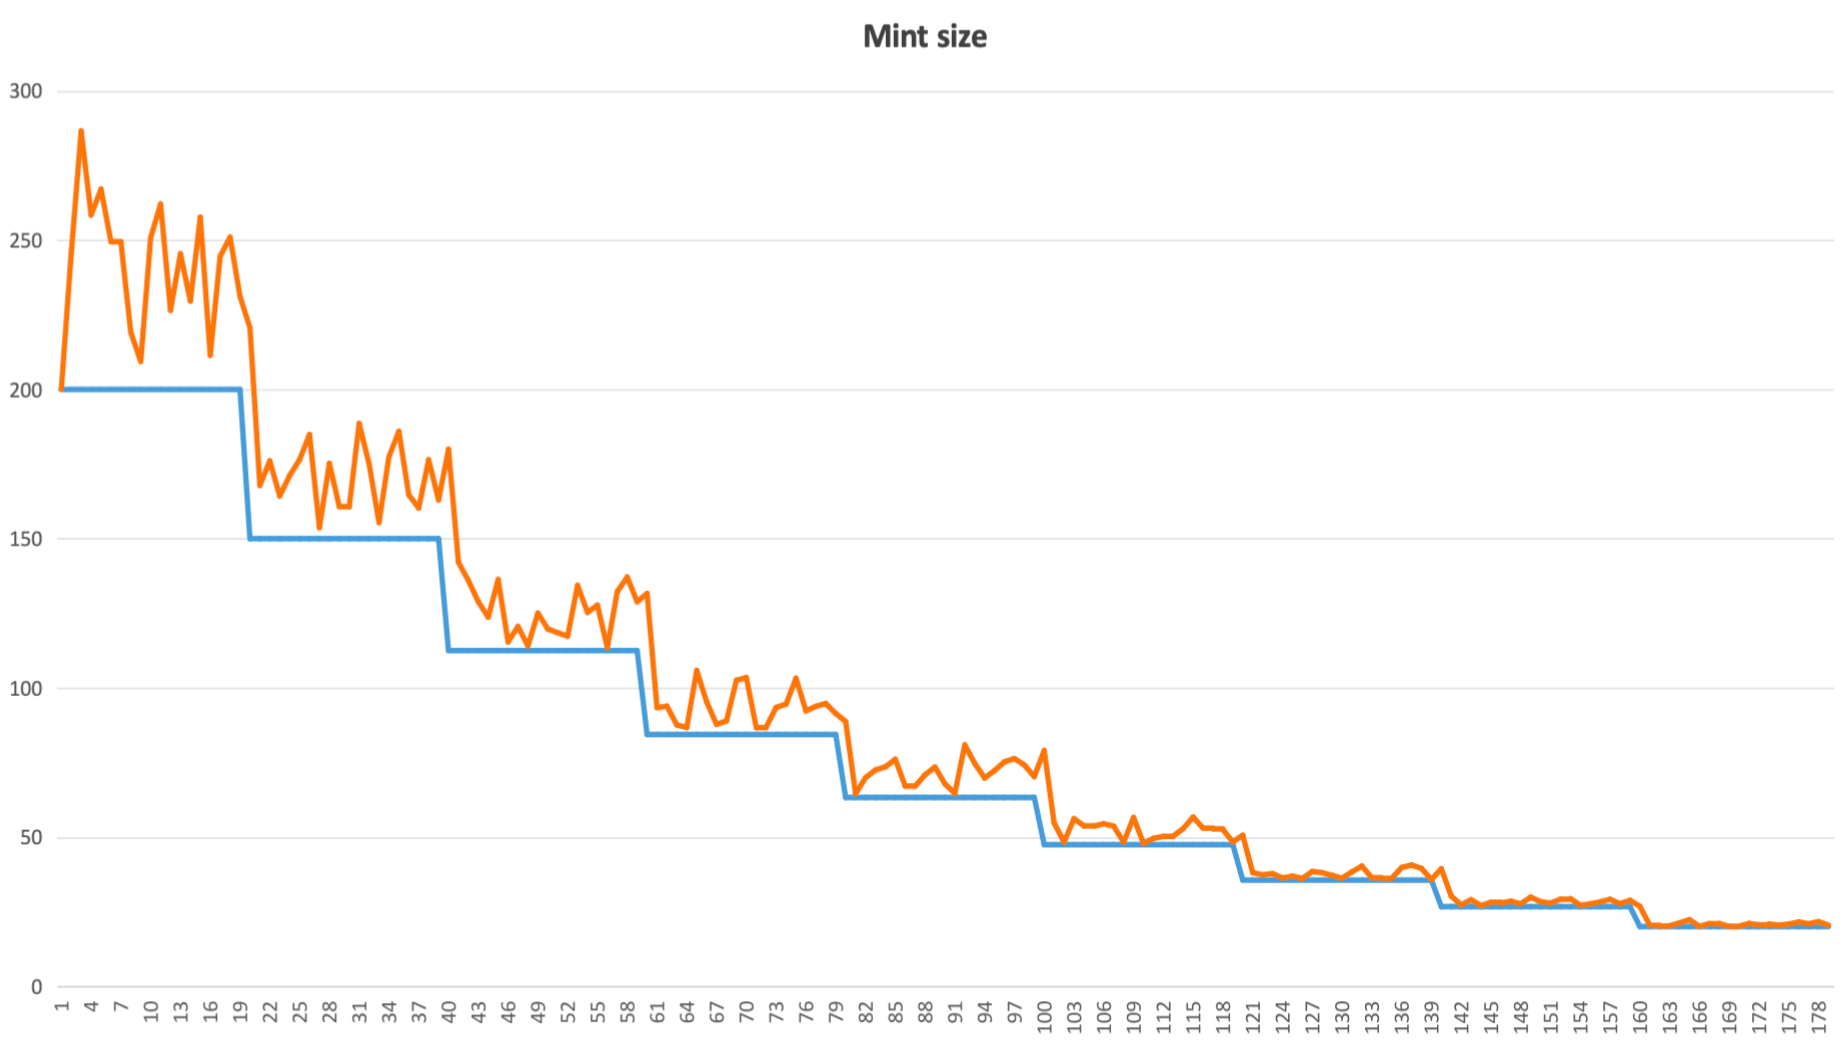
\includegraphics[width=400px]{image}

週期實際鑄造收益同目標鑄造收益對比

橙色線條係\textbf{當前週期嘅實際鑄造規模},藍色線條係\textbf{每次鑄造嘅目標鑄造規模},顯示每個時代減少25\%嘅趨勢。

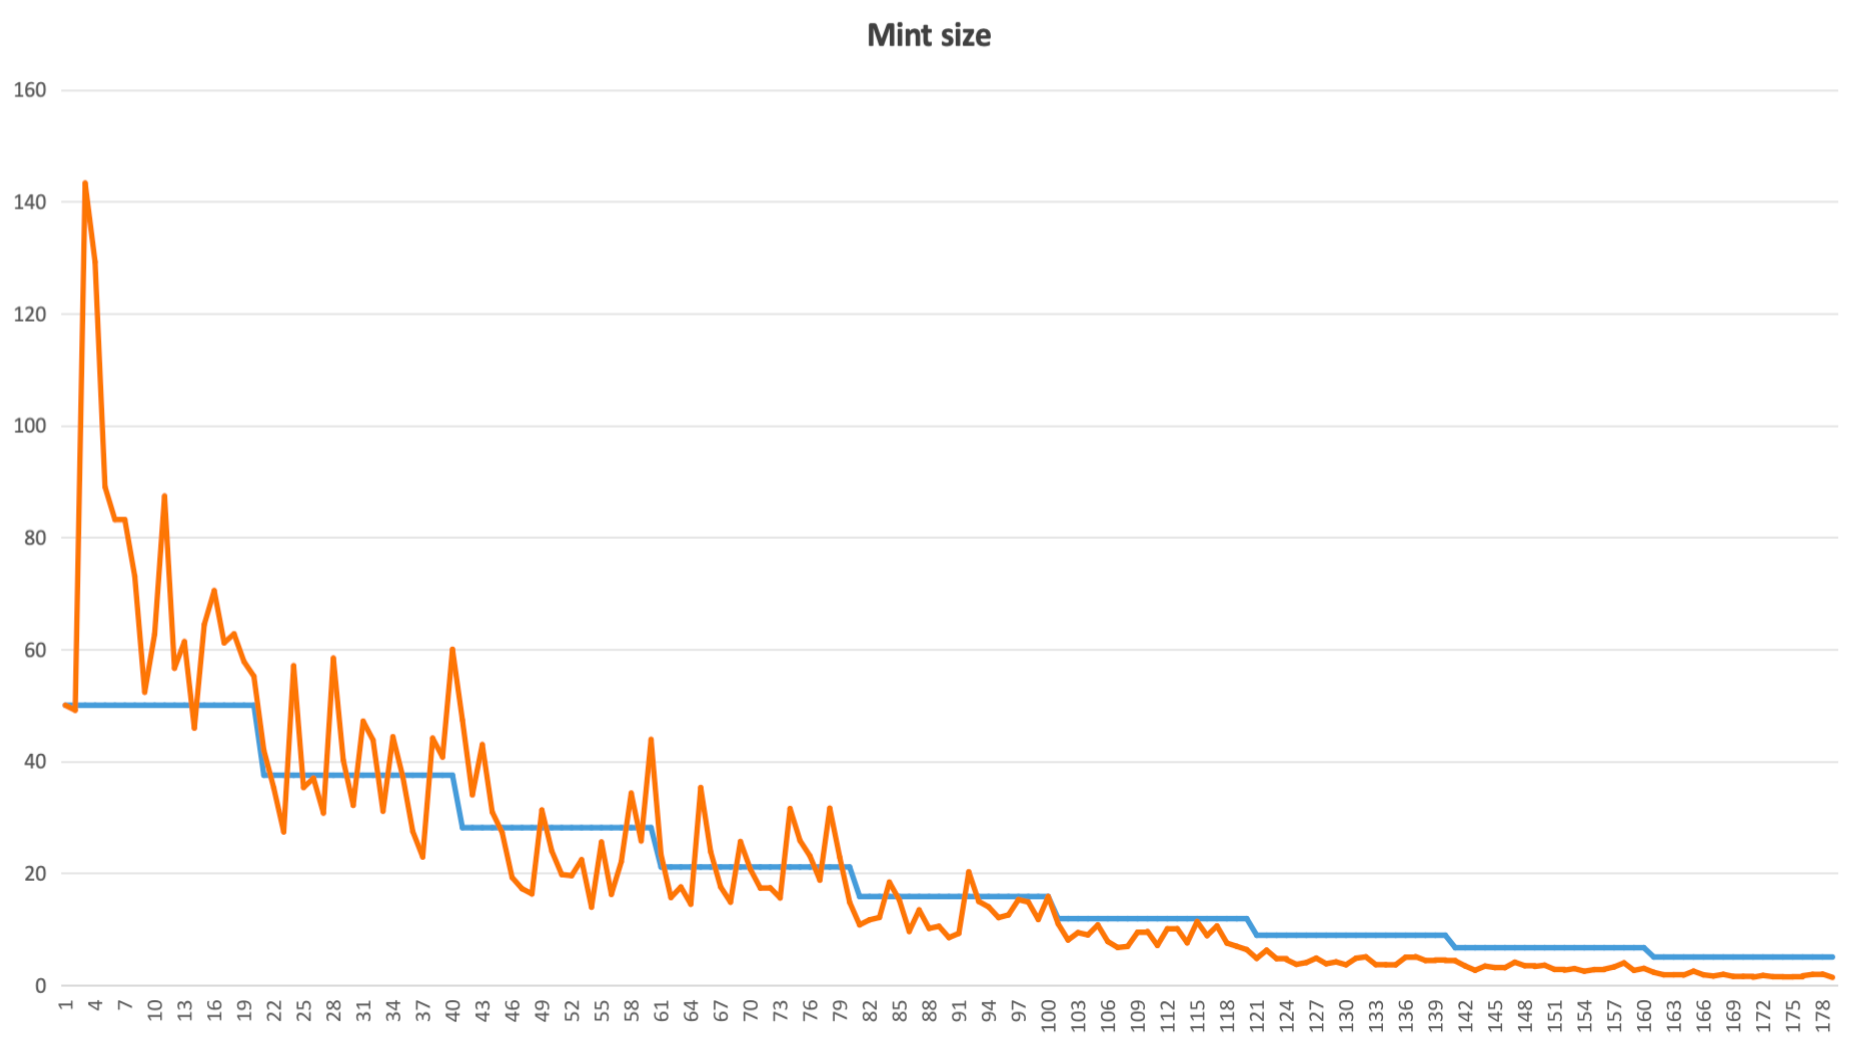
\includegraphics[width=400px]{image1}

實際鑄造獎勵同目標鑄造獎勵

橙色線條係\textbf{實際鑄造規模},藍色線條係\textbf{目標鑄造規模}。

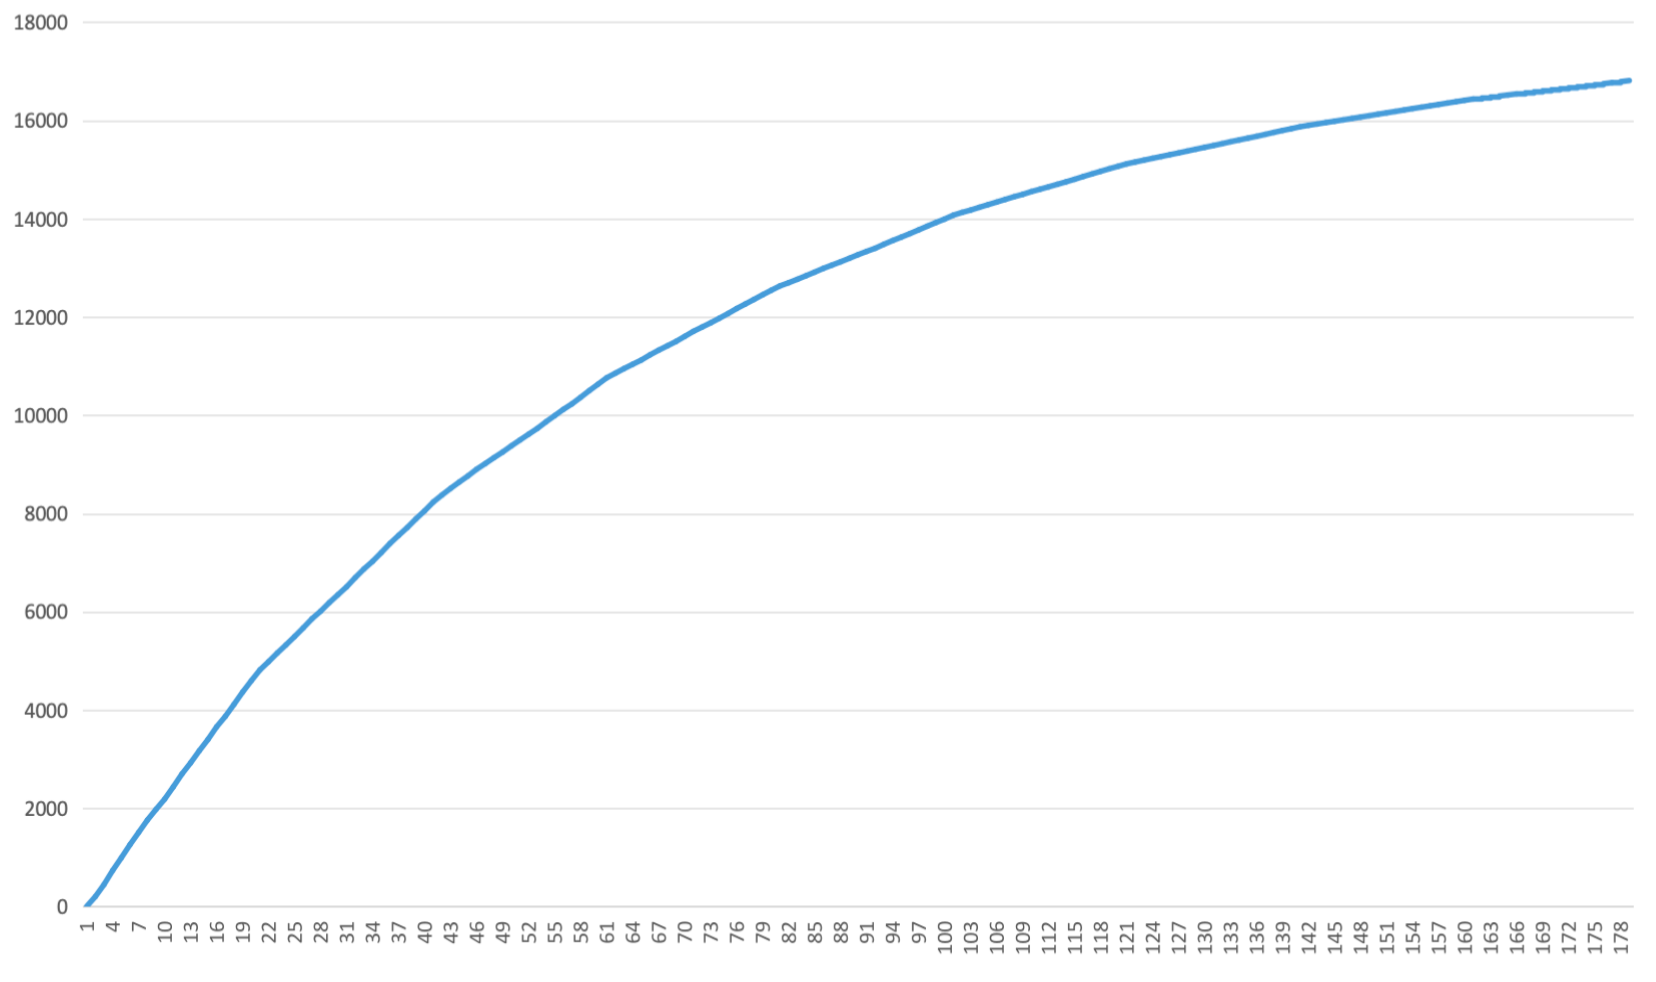
\includegraphics[width=400px]{image2}

總鑄造曲線

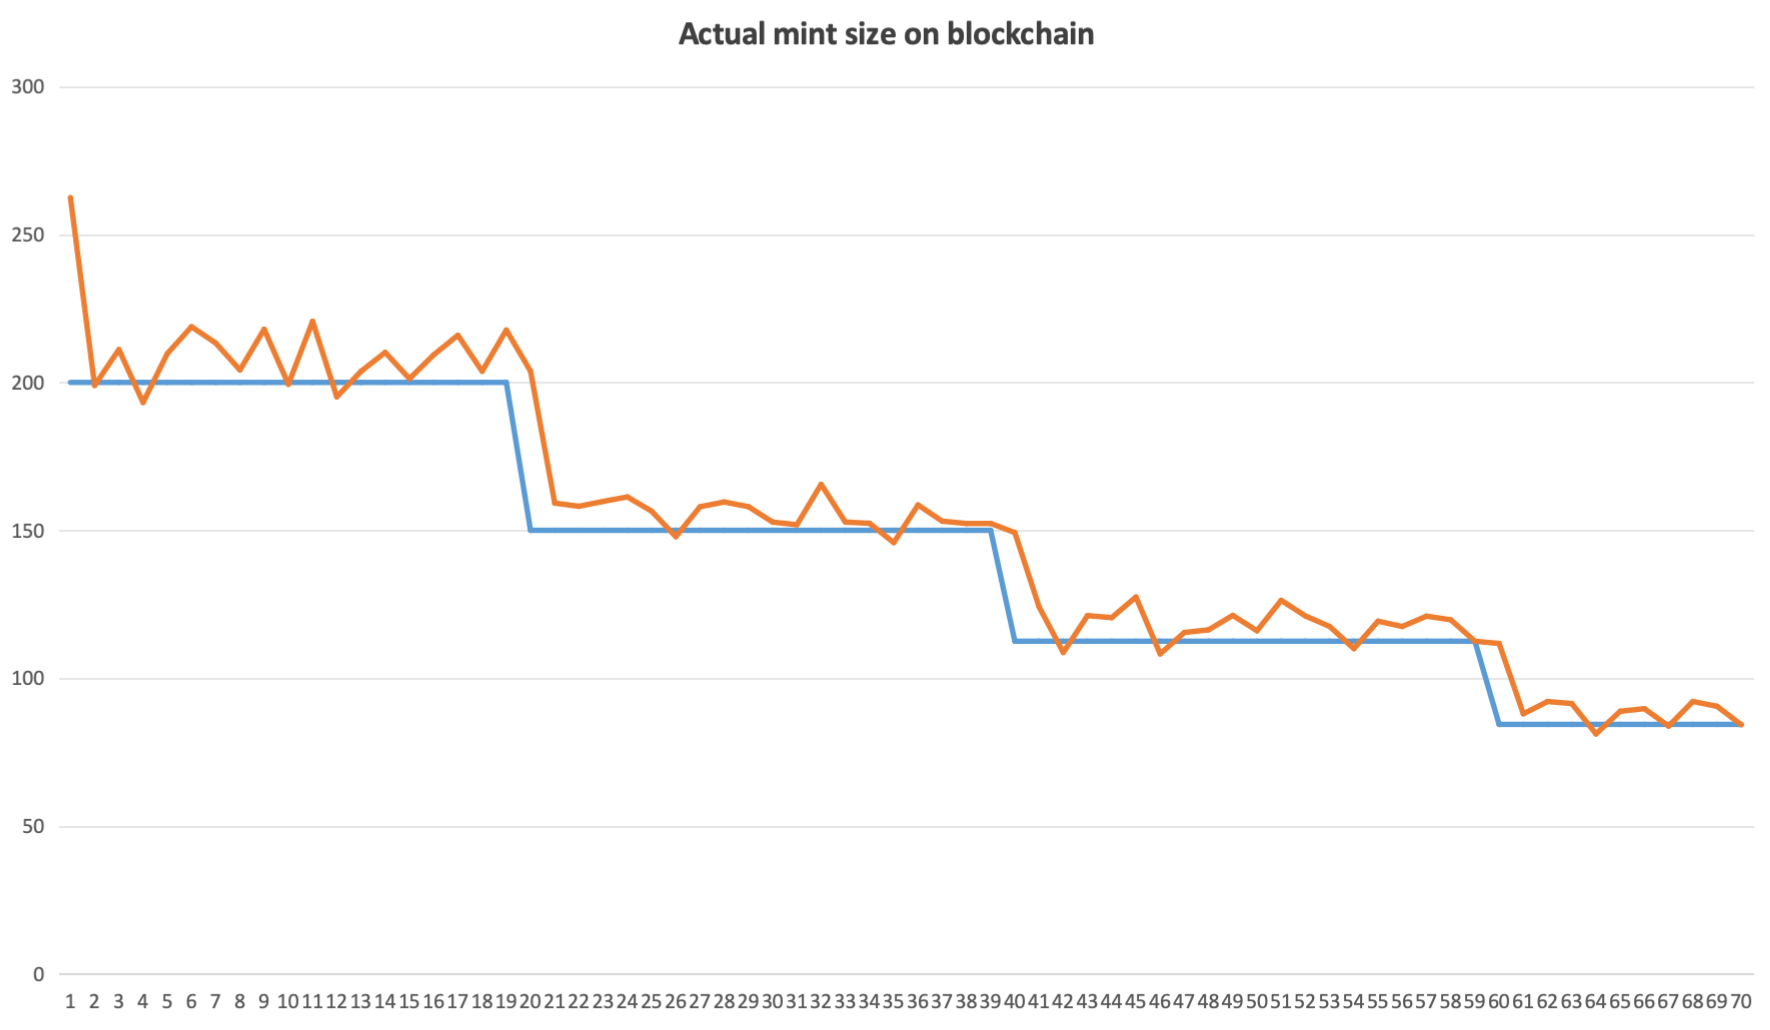
\includegraphics[width=400px]{image3}

以太坊鏈上嘅模擬結果

以上係喺以太坊鏈上嘅模擬結果。

\subsection{6. 聯盟鑄造計劃}\label{ux806fux76dfux9444ux9020ux8a08ux5283}

\subsubsection{6.1 - 描述}\label{ux63cfux8ff0}

\textbf{聯盟鑄造計劃}(\textbf{AMP})允許每個用戶生成一個\textbf{唯一推薦碼}(\textbf{URC})同其他人分享。當其他人使用呢個\textbf{URC}進行鑄造時,佢哋可以獲得鑄造費用嘅折扣,推薦者可以獲得一啲獎勵。\textbf{AMP}設計為去中心化同社群驅動,激勵建立更好嘅社群。

\begin{enumerate}
\def\labelenumi{\arabic{enumi}.}
\tightlist
\item
  去中心化同社群驅動

  \begin{itemize}
  \tightlist
  \item
    所有鑄造必須使用\textbf{URC},每次鑄造都同社群中嘅某個成員相關聯。
  \item
    鑄造嘅進度同速度受社群成員分享\textbf{URC}嘅影響,而唔係由核心團隊或某些大戶控制。
  \item
    透過\textbf{AMP},社群更容易形成共識同吸引更多成員參與社群。
  \end{itemize}
\item
  激勵社群

  \begin{itemize}
  \tightlist
  \item
    雙重激勵:推薦者(代碼分享者)同使用\textbf{URC}嘅鑄造者都可以受益,呢個雙重激勵機制有助於社群嘅增長同活躍度。
  \end{itemize}
\item
  鑄造折扣同推薦者獎勵

  \begin{itemize}
  \tightlist
  \item
    鑄造費用折扣同提供\textbf{URC}嘅帳戶嘅代幣餘額掛鈎。推薦者嘅餘額越多,鑄造折扣越高,鑄造費用越低。呢個會鼓勵參與者持有更多代幣而唔係全部賣出。
  \item
    \textbf{URC}分享者可以獲得穩定嘅獎勵,呢啲獎勵喺鑄造發生時由鏈上貨幣(以太坊嘅ETH或Solana嘅SOL)自動分配到推薦者嘅帳戶。
  \end{itemize}
\item
  鑄造費用同難度調整

  \begin{itemize}
  \tightlist
  \item
    動態難度:鑄造嘅總成本同難度會根據社群動態調整;鑄造人數越多,鑄造速度越快,總鑄造成本越高,額外鑄造費用亦越高。
  \item
    部分鑄造費用會作為折扣重新分配畀鑄造者同作為獎勵畀\textbf{URC}分享者。
  \end{itemize}
\end{enumerate}

\begin{equation}
ExtraMintFee = \frac{P_0 \cdot T_0}{M_0} \cdot (\sum_{i=0}^{C_e}d_i - C_e - 1)
\end{equation}
呢個公式表明,\(d_i\)越高(大約高於1),額外鑄造費用越高。

由於鑄造費用進入流動性池以支持市場交易,因此\textbf{AMP}會對社群發展同代幣交易產生積極影響。

\subsubsection{6.2 - 計算}\label{ux8a08ux7b97-1}

\paragraph{6.2.1 - 鑄造折扣}\label{ux9444ux9020ux6298ux6263}

折扣由代碼分享者嘅餘額同代幣總供應量嘅比例決定。

\begin{itemize}
\tightlist
\item
  \(r\):代碼分享者嘅餘額同\textbf{當前}代幣總供應量嘅比例。
\item
  \(k\):折扣率。
\end{itemize}

\begin{longtable}[]{@{}ll@{}}
\toprule\noalign{}
\(r\) & \(k\) \\
\midrule\noalign{}
\endhead
\bottomrule\noalign{}
\endlastfoot
\textless{} 0.2\% & 0 \\
0.2-0.4\% & 5\% \\
0.4-0.6\% & 10\% \\
0.6-0.8\% & 15\% \\
0.8-1\% & 20\% \\
\textgreater{} 1\% & 25\% \\
\end{longtable}

\paragraph{6.2.2 -
折扣後嘅鑄造費用}\label{ux6298ux6263ux5f8cux5605ux9444ux9020ux8cbbux7528}

\begin{itemize}
\tightlist
\item
  \(Fee\):折扣後嘅鑄造費用
\item
  \(P_0\):原始鑄造費用
\item
  \(p_0\):第一個週期鑄造代幣嘅價格
\item
  \(p\):折扣前嘅鑄造代幣價格
\item
  \(d\):難度係數
\item
  \(k\):折扣率
\end{itemize}

\begin{equation}
\frac{Fee}{M_b} \cdot d = p_0 + (p - p_0) \cdot (1 - k) = p \cdot (1 - k) + p_0 \cdot k
\end{equation} \begin{equation}
p = \frac{P_0}{M_b} \cdot d, p_0 = \frac{P_0}{M_b}
\end{equation}

從上述等價公式,我哋可以得到折扣後嘅鑄造費用: \begin{equation}
Fee = P_0 \cdot (1 + \frac{k}{d} - k),  (d \geq 1, k \leq 0.25)
\end{equation}

\(Fee\)同原始\(P_0\)之間嘅差額為: \begin{equation}
P_0 - Fee = P_0 - P_0 \cdot (1 + \frac{k}{d} - k) = P_0 \cdot k \cdot (1 - \frac{1}{d})
\end{equation}

折扣率為: \begin{equation}
\frac{P_0-Fee}{P_0} =k \cdot (1 - \frac{1}{d})
\end{equation}

\textbf{示例:}

\(P_0=8\)美元, \(d=12.3\), \(Token Balance\)=26,000, \(Total Supply\) =
5,000,000美元

代幣佔總供應量嘅比例(\(r\)) = 26,000 / 5,000,000 = 0.52\%,

因此折扣(\(k\))為10\%。

實際鑄造費用為:\(8 * (1 + 0.1 / 12.3 - 0.1) = 7.265\)美元

同原始鑄造費用相比,折扣為: \(1 - 7.265 / 8 = 9.19\)\%

\paragraph{6.2.3 -
唯一推薦碼(URC)}\label{ux552fux4e00ux63a8ux85a6ux78bcurc}

唯一推薦碼(URC)係由分享者嘅帳戶同時間戳生成嘅唯一代碼。

\paragraph{6.2.4 -
推薦碼嘅限制}\label{ux63a8ux85a6ux78bcux5605ux9650ux5236}

\begin{itemize}
\item
  推薦碼嘅使用次數唔係無限,預設為50。呢個意味着喺呢個代碼被用咗\textbf{50}次鑄造後,代碼會失效,分享者需要重新激活。
\item
  代碼分享者唔可以隨時重新激活代碼,每次激活之間有間隔。預設間隔為\textbf{24小時}。
\end{itemize}

\paragraph{6.2.5 -
代碼分享者嘅收益}\label{ux4ee3ux78bcux5206ux4eabux8005ux5605ux6536ux76ca}

代碼分享者可以攞到鑄造者節省嘅費用餘額嘅20\%。

\begin{equation}
CodeSharerReward = 0.2 \cdot (P_0 - Fee) = 0.2 \cdot P_0 \cdot k \cdot (1 - \frac{1}{d})
\end{equation}

難度越高,\(k\)越大,代碼分享者嘅收益越大。

\textbf{示例:}

從之前嘅示例,代碼分享者嘅獎勵為:

\(0.2 * 8 * 0.10 * (1 - 1/12.3) = 0.147\)美元

\subsubsection{6.3 - 評估}\label{ux8a55ux4f30}

我哋嚟改動一下鑄造費用嘅公式,睇下佢點樣影響費用。 \begin{equation}
\frac{MintFee}{P_0} = 1 + \frac{k}{d} - k, (d \geq 1, k \leq 0.25)
\end{equation}

\paragraph{\texorpdfstring{6.3.1 -
難度(\(d\))對鑄造費用嘅影響}{6.3.1 - 難度(d)對鑄造費用嘅影響}}\label{ux96e3ux5ea6dux5c0dux9444ux9020ux8cbbux7528ux5605ux5f71ux97ff}

根據鑄造費用嘅公式,難度越高,鑄造費用越低,折扣越多。

\paragraph{\texorpdfstring{6.3.2 -
\(k\)對鑄造費用嘅影響}{6.3.2 - k對鑄造費用嘅影響}}\label{kux5c0dux9444ux9020ux8cbbux7528ux5605ux5f71ux97ff}

根據鑄造費用嘅公式,\(k\)越高,鑄造費用越低,折扣越多。

\paragraph{6.3.3 - 風險}\label{ux98a8ux96aa}

我哋要考慮一個情況,\textbf{AMP}可能會導致自我鑄造(用自己嘅\textbf{URC}進行鑄造),但我哋相信:一旦一個人擁有一定數量嘅代幣,佢哋會更傾向於建立社群同同其他人分享代碼。

另外,即使每個人都用最大折扣進行鑄造(呢個係唔可能嘅),最低總鑄造費用會如下:

\begin{equation}
CodeSharerReward = 0.2 \cdot (P_0 - Fee) = 0.2 \cdot P_0 \cdot k \cdot (1 - \frac{1}{d})
\end{equation}

因為\(max(k)\) = 25\%,當\(d = \infty\)時,代碼分享者收到\(P_0\)嘅5\%。

所以,最低總鑄造費用係計劃嘅95\%。考慮到\textbf{AMP}可能帶來嘅社群活躍度,以及難度嘅增加會提高鑄造費用,呢個減少係值得嘅。

\subsubsection{6.4 - 初始化}\label{ux521dux59cbux5316}

\paragraph{6.4.1 - 系統推薦者}\label{ux7cfbux7d71ux63a8ux85a6ux8005}

點解需要系統/默認推薦者?

所有鑄造都需要\textbf{URC},如果有人唔能夠從社群成員嗰度得到\textbf{URC},佢可以是用系統提供嘅默認\textbf{URC}。

用默認\textbf{URC}時,無折扣(因為默認推薦者嘅帳戶餘額為0)。

\subsubsection{6.5 - 計劃實現}\label{ux8a08ux5283ux5be6ux73fe}

\begin{Shaded}
\begin{Highlighting}[numbers=left,,]
\CommentTok{// Calculate the fee value and the referrer reward}
\KeywordTok{pub} \KeywordTok{fn}\NormalTok{ get\_fee\_value(fee\_rate}\OperatorTok{:} \DataTypeTok{u64}\OperatorTok{,}\NormalTok{ difficulty\_coefficient}\OperatorTok{:} \DataTypeTok{f64}\OperatorTok{,}\NormalTok{ referrer\_ata\_balance}\OperatorTok{:} 
  \DataTypeTok{u64}\OperatorTok{,}\NormalTok{ total\_supply}\OperatorTok{:} \DataTypeTok{f64}\NormalTok{) }\OperatorTok{{-}\textgreater{}}\NormalTok{ (}\DataTypeTok{f64}\OperatorTok{,} \DataTypeTok{f64}\NormalTok{) }\OperatorTok{\{}
  \KeywordTok{let}\NormalTok{ balance\_ratio }\OperatorTok{=}\NormalTok{ referrer\_ata\_balance }\KeywordTok{as} \DataTypeTok{f64} \OperatorTok{/}\NormalTok{ total\_supply}\OperatorTok{;}
  \KeywordTok{let}\NormalTok{ discount\_rate }\OperatorTok{=} \ControlFlowTok{if}\NormalTok{ balance\_ratio }\OperatorTok{\textless{}} \DecValTok{0.002} \OperatorTok{\{}\DecValTok{0.0}\OperatorTok{\}}
  \ControlFlowTok{else} \ControlFlowTok{if}\NormalTok{ balance\_ratio }\OperatorTok{\textless{}} \DecValTok{0.004} \OperatorTok{\{}\DecValTok{0.05}\OperatorTok{\}}
  \ControlFlowTok{else} \ControlFlowTok{if}\NormalTok{ balance\_ratio }\OperatorTok{\textless{}} \DecValTok{0.006} \OperatorTok{\{}\DecValTok{0.1}\OperatorTok{\}}
  \ControlFlowTok{else} \ControlFlowTok{if}\NormalTok{ balance\_ratio }\OperatorTok{\textless{}} \DecValTok{0.008} \OperatorTok{\{}\DecValTok{0.15}\OperatorTok{\}}
  \ControlFlowTok{else} \ControlFlowTok{if}\NormalTok{ balance\_ratio }\OperatorTok{\textless{}} \DecValTok{0.01} \OperatorTok{\{}\DecValTok{0.2}\OperatorTok{\}}
  \ControlFlowTok{else} \OperatorTok{\{}\DecValTok{0.25}\OperatorTok{\};}
  \KeywordTok{let}\NormalTok{ fee }\OperatorTok{=}\NormalTok{ fee\_rate }\KeywordTok{as} \DataTypeTok{f64} \OperatorTok{*}\NormalTok{ (}\DecValTok{1.0} \OperatorTok{+}\NormalTok{ discount\_rate }\OperatorTok{/}\NormalTok{ difficulty\_coefficient }\OperatorTok{{-}} 
\NormalTok{    discount\_rate)}\OperatorTok{;}
  \KeywordTok{let}\NormalTok{ code\_sharer\_reward }\OperatorTok{=} \DecValTok{0.2} \OperatorTok{*}\NormalTok{ fee\_rate }\KeywordTok{as} \DataTypeTok{f64} \OperatorTok{*}\NormalTok{ discount\_rate }\OperatorTok{*}\NormalTok{ (}\DecValTok{1.0} \OperatorTok{{-}} \DecValTok{1.0} \OperatorTok{/} 
\NormalTok{    difficulty\_coefficient)}\OperatorTok{;}
\NormalTok{  (fee }\KeywordTok{as} \DataTypeTok{f64}\OperatorTok{,}\NormalTok{ code\_sharer\_reward)}
\OperatorTok{\}}
\end{Highlighting}
\end{Shaded}

\subsubsection{6.6 -
URC生成同驗證流程}\label{urcux751fux6210ux540cux9a57ux8b49ux6d41ux7a0b}

為咗避免機械人監控URC代碼嘅生成同更新以進行搶跑,前端同區塊鏈之間只交換\textbf{URC\_Pubkey}。

以下係Solana區塊鏈上URC生成同驗證嘅流程。

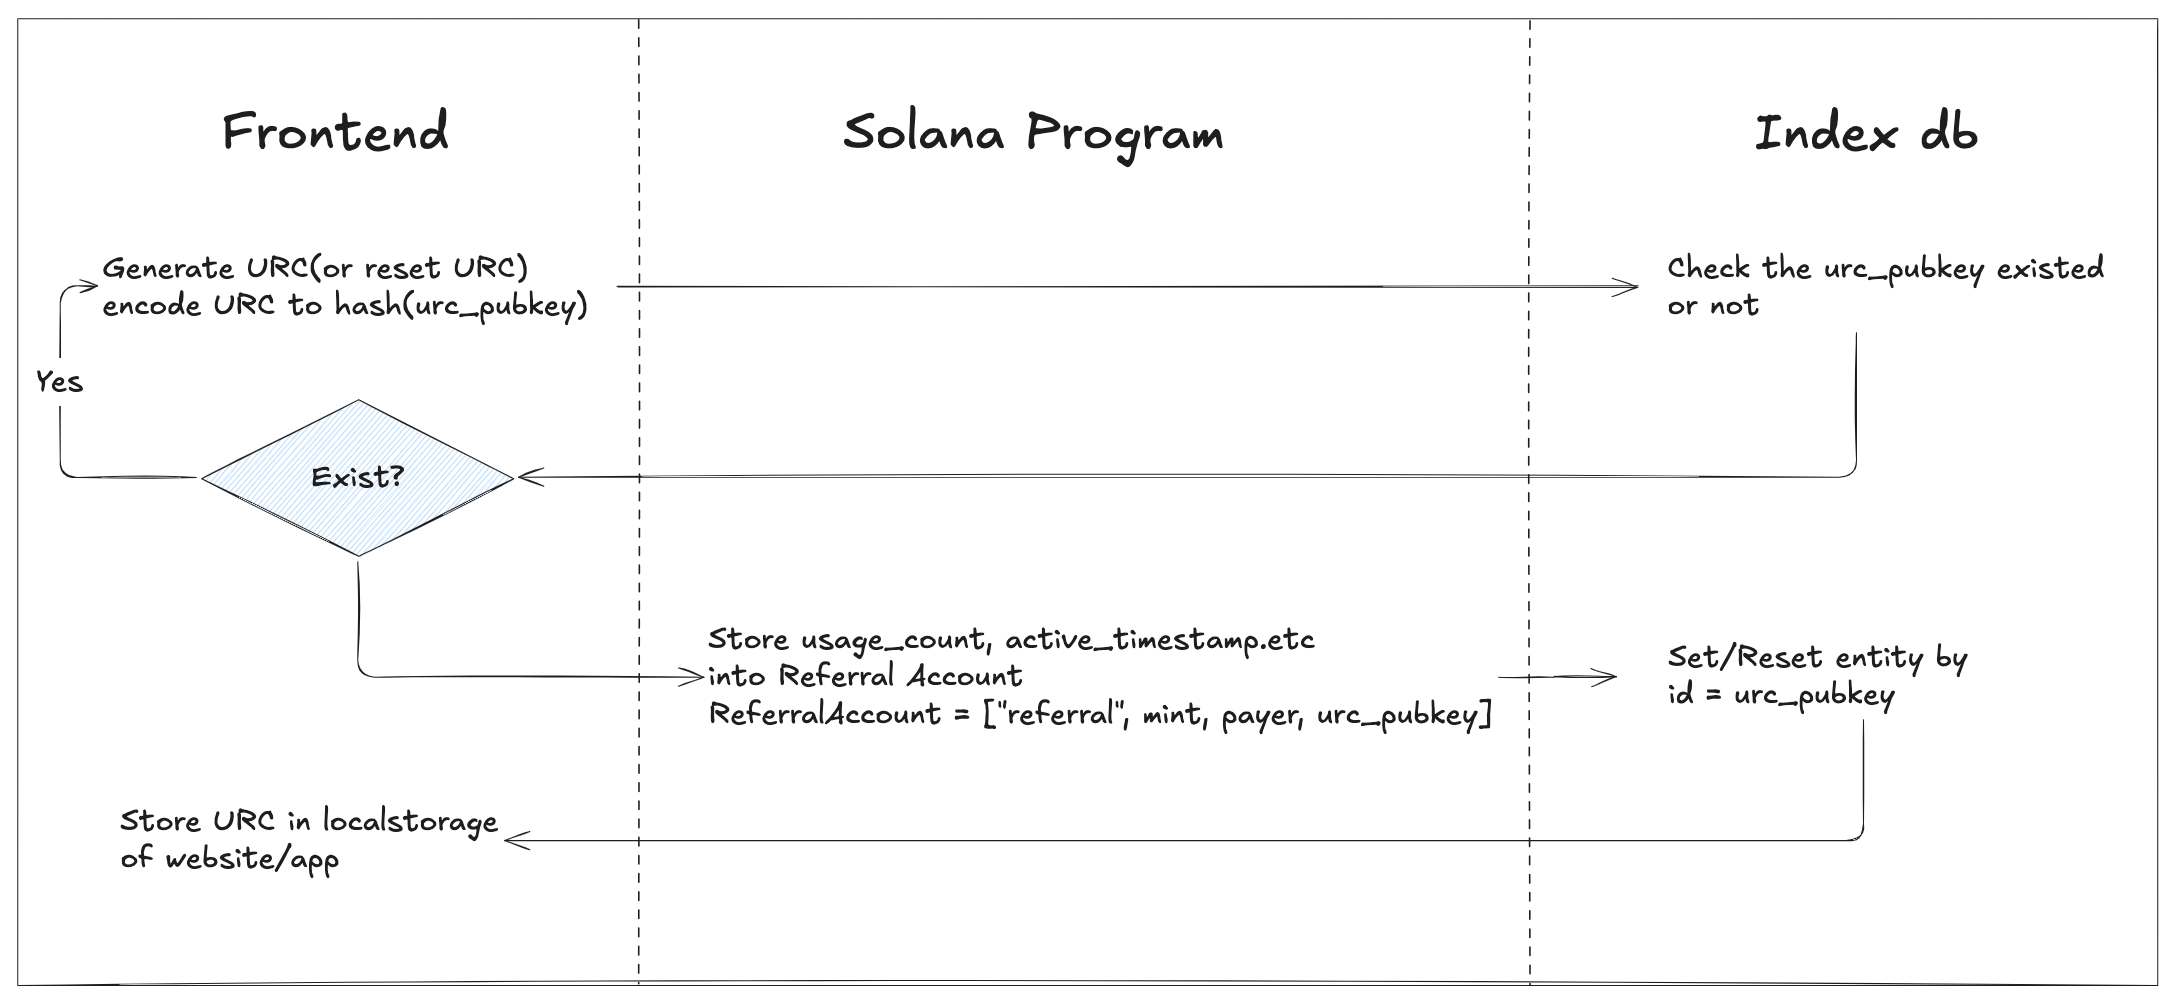
\includegraphics[width=400px]{urc_workflow}

\subsection{7 - 流動性}\label{ux6d41ux52d5ux6027}

鑄造費用最終會注入去中心化交易所嘅流動性池,喺嗰度可以賺取交易費用。

\subsubsection{7.1 -
流動性池嘅代幣}\label{ux6d41ux52d5ux6027ux6c60ux5605ux4ee3ux5e63}

總代幣供應量嘅一部分會分配畀流動性池,作為SOL/代幣對。呢部分分配喺鑄造期間進入專用流動性帳戶。一旦滿足某些條件(例如,第一個時代完成),呢啲代幣連同交易費用(SOL)會自動加入流動性池。

\begin{itemize}
\tightlist
\item
  \(M_a\):每次鑄造嘅代幣數量(見3.1.4,3.1.4)
\item
  \(r_l\):初始流動性池相對於總發行量嘅比例,\(r_l < 1\)
\item
  \(L\):每次鑄造事件進入流動性專用帳戶嘅代幣數量
\end{itemize}

\begin{equation}
L = \frac{M_a \cdot r_l}{1 - r_l}
\end{equation}

因為代幣總供應量為: \begin{equation}
TotalSupply = \sum_{i=1}^{E}(C \cdot T_0 \cdot \frac{1-f^{E}}{1-f})=C \cdot T_0 \cdot \frac{1-f^{E}}{1-f}
\end{equation}

初始化流動性池嘅代幣為:

\begin{equation}
InitLiquidity = TotalSupply * \frac{r_l}{1-r_l} = C \cdot T_0 \cdot r_l \cdot \frac{1-f^{E}}{(1-f) \cdot (1-r_l)}
\end{equation}

\subsubsection{7.2 - 鑄造費用}\label{ux9444ux9020ux8cbbux7528}

鑄造費用喺6.2.2節有描述。鑄造費用嘅分配如下:

\begin{itemize}
\tightlist
\item
  URC提供者:0-5\%
\item
  協議費用:5\%
\item
  流動性池:90-95\%
\end{itemize}

\subsubsection{7.3 -
初始化流動性池時嘅預計價格}\label{ux521dux59cbux5316ux6d41ux52d5ux6027ux6c60ux6642ux5605ux9810ux8a08ux50f9ux683c}

根據去中心化交易所嘅\textbf{AMM},初始化流動性池時嘅代幣價格為:

\begin{equation}
Price = \frac{0.90 \cdot TotalFee}{InitLiquidity}
\end{equation}

由於總鑄造費用係一個範圍: \begin{equation}
TotalFee \in [\frac{P_0 \cdot T_0}{M_0} \cdot C_e, \frac{P_0 \cdot T_0}{M_0} \cdot 101 \cdot (1.01^{C_e}-1)]
\end{equation}

所以,初始化流動性池時嘅最低價格為: \begin{equation}
P_{low} = \frac{P_0 \cdot C_e \cdot (1-r_l)(1-f)}{M_0 \cdot C \cdot r_l \cdot (1-f^E)}*0.90
\end{equation}

最高價格為: \begin{equation}
P_{high} = \frac{101 \cdot P_0 \cdot (1.01^{C_e}-1)(1-r_l)(1-f)}{M_0 \cdot C \cdot r_l \cdot (1-f^E)}*0.90=\frac{101 \cdot (1.01^{C_e}-1)}{C_e} \cdot P_{low}
\end{equation}

喺上述公式中,\(C_e = E \cdot C\)(\(C\)係每個時代嘅週期數,\(E\)係時代數)

\subsection{8 退款}\label{ux9000ux6b3e}

鑄造證明(PoM)係一個根據時間動態調整鑄造規模嘅新代幣發行模式。其核心邏輯如下:

\begin{itemize}
\tightlist
\item
  \textbf{動態成本調整}:

  \begin{itemize}
  \tightlist
  \item
    當實際鑄造時間\textbf{短於目標鑄造時間}時,鑄造規模減少,代幣成本增加。
  \item
    當實際鑄造時間\textbf{等於或長於目標鑄造時間}時,鑄造數量同代幣成本保持不變。
  \end{itemize}
\item
  \textbf{激勵機制}:

  \begin{itemize}
  \tightlist
  \item
    呢個機制透過成本增加激勵早期參與者,推動鑄造活動。
  \item
    但係,佢亦可能導致後期參與者嘅成本過高,影響公平性。
  \end{itemize}
\end{itemize}

\subsubsection{8.1
退款機制嘅介紹同設計}\label{ux9000ux6b3eux6a5fux5236ux5605ux4ecbux7d39ux540cux8a2dux8a08}

為咗解決上述問題,PoM引入咗\textbf{退款}作為輔助約束,以確保公平性同保護參與者。其關鍵點如下:

\paragraph{8.1.1
目標時代鎖定:}\label{ux76eeux6a19ux6642ux4ee3ux9396ux5b9a}

喺目標時代期間,所有籌集嘅鑄造費用都被鎖定喺一個特殊金庫入面,參與者可以隨時發起退款。

\paragraph{8.1.2
代幣數量驗證:}\label{ux4ee3ux5e63ux6578ux91cfux9a57ux8b49}

退款時,系統會驗證用戶錢包中嘅代幣總量係咪等於鑄造時嘅數量。

如果用戶已經轉移或交易咗部分代幣,除非喺錢包中補充相應數量嘅代幣,否則退款會失敗。

\paragraph{8.1.3
費用扣除規則:}\label{ux8cbbux7528ux6263ux9664ux898fux5247}

退款時,會扣除部分貨幣(例如,ETH/SOL)作為退款費用,以防止濫用。

如果喺鑄造時使用咗URC並獲得折扣,退款時會扣除已支付畀URC提供者嘅獎勵。

\paragraph{8.1.4
退款嘅優點同效果}\label{ux9000ux6b3eux5605ux512aux9edeux540cux6548ux679c}

\begin{itemize}
\tightlist
\item
  \textbf{公平性保障}:

  \begin{itemize}
  \tightlist
  \item
    透過退款,後期參與者唔需要承擔過高嘅鑄造成本,確保公平參與。
  \item
    鑄造費用嘅動態調整同退款機制一齊作用,避免因``熱鑄造''導致嘅成本激增。
  \end{itemize}
\item
  \textbf{防止女巫攻擊}:

  \begin{itemize}
  \tightlist
  \item
    由於後期參與者可能會發起退款,女巫攻擊者喺早期干預嘅動機被削弱。
  \item
    呢個機制透過經濟激勵同約束有效降低惡意行為嘅概率。
  \end{itemize}
\item
  \textbf{社群模擬驗證}:

  \begin{itemize}
  \tightlist
  \item
    社群內進行嘅模擬測試顯示,退款顯著提高咗鑄造過程嘅公平性同參與者滿意度。
  \item
    最直接嘅結果係,由於退款風險,女巫攻擊者減少咗惡意活動,進一步優化咗生態系統嘅健康。
  \end{itemize}
\end{itemize}

\subsubsection{8.2
退款唔係隨時可用}\label{ux9000ux6b3eux5514ux4fc2ux96a8ux6642ux53efux7528}

請注意,退款只喺目標時代期間可用。目標時代結束後,鑄造費用會用於初始化流動性池,退款功能會被禁用。

\subsection{9 -
完整案例研究}\label{ux5b8cux6574ux6848ux4f8bux7814ux7a76}

以下係喺\textbf{Solana}區塊鏈上部署鑄造證明(PoM)機制嘅全面案例研究。

\subsubsection{9.1 - 參數}\label{ux53c3ux6578}

\begin{itemize}
\tightlist
\item
  總供應量:1,000,000,000代幣
\item
  第一個時代每次鑄造嘅目標規模(\(M_0\)):10,000代幣
\item
  第一個時代每個週期嘅目標鑄造規模(\(T_0\)):1,000,000代幣
\item
  每個週期嘅最小鑄造實例數:100
\item
  目標時代(\(E\)):1,第一個時代完成後,持有者可以轉移代幣,流動性池初始化。
\item
  每個時代嘅週期數(\(C\)):250
\item
  目標鑄造天數:30天
\item
  減少因子(\(f\)):0.75
\item
  流動性代幣百分比(\(r_l\)):10\%
\item
  每次鑄造嘅費用(\(P_0\)):2美元每次鑄造(0.0002美元/代幣)
\item
  每個週期嘅目標鑄造時間:173分鐘(大約3小時)
\item
  初始化流動性池時生成嘅LP代幣嘅處理方式:\textbf{全部銷毀}
\item
  達到目標時代\#1時:

  \begin{itemize}
  \tightlist
  \item
    總供應量:250,000,000代幣(最大供應量嘅25\%)
  \item
    總週期數:250
  \item
    鑄造次數:\textgreater= 25,000
  \item
    總鑄造費用:50,200美元至223,050美元
  \item
    初始化流動性池時嘅價格:0.001807美元至0.008030美元
  \end{itemize}
\end{itemize}

\subsubsection{9.2 -
鑄造流程(技術上)}\label{ux9444ux9020ux6d41ux7a0bux6280ux8853ux4e0a}

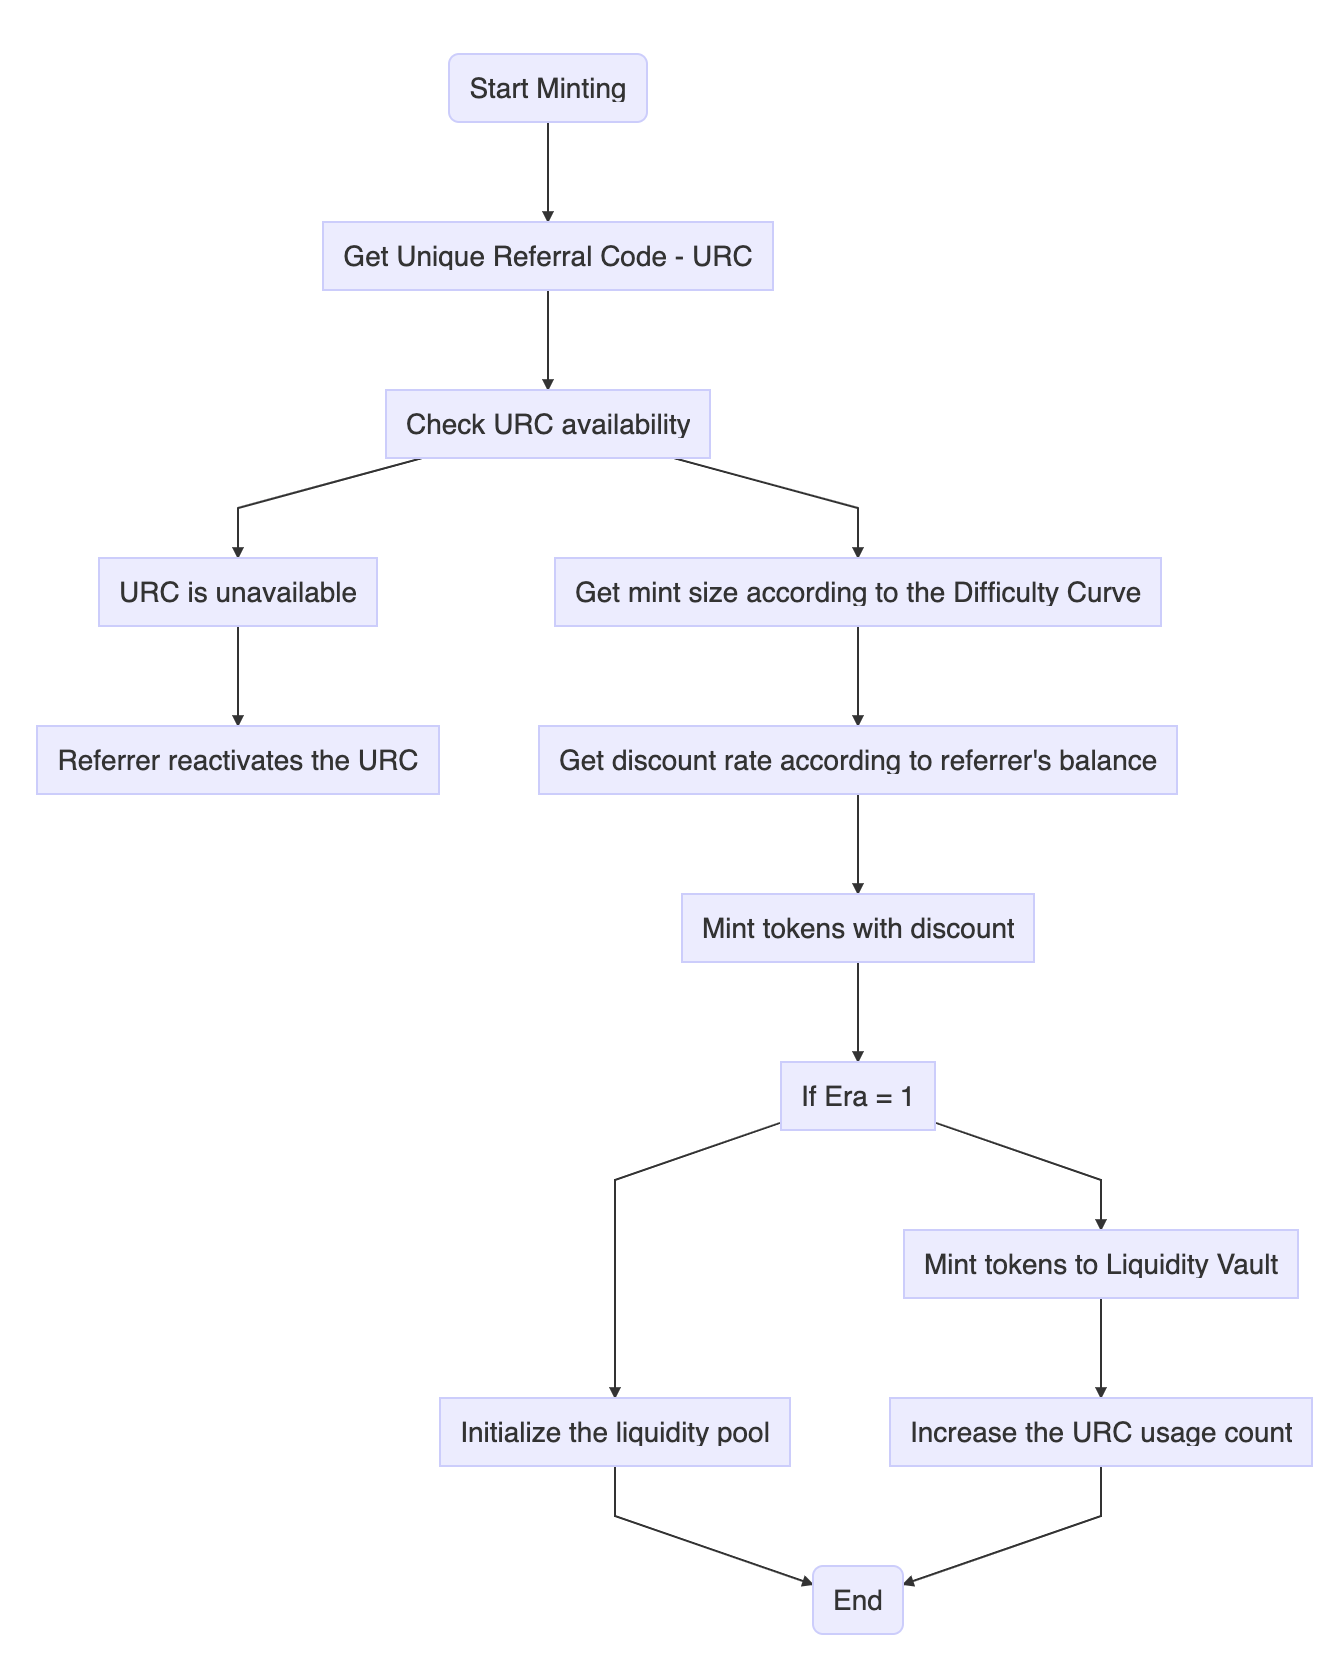
\includegraphics[width=400px]{mint_workflow}

\subsubsection{9.3 -
初始化流動性池流程(技術上)}\label{ux521dux59cbux5316ux6d41ux52d5ux6027ux6c60ux6d41ux7a0bux6280ux8853ux4e0a}

任何人都可以初始化流動性,唯一條件係時代 \textgreater{} 1。

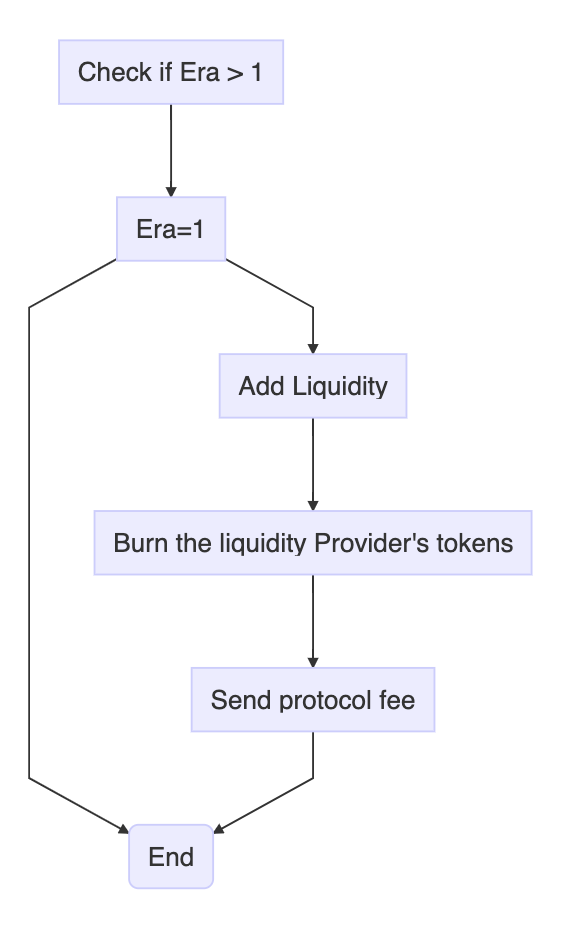
\includegraphics[width=200px]{initialize_liquidity_workflow}

\end{document}
